\documentclass[twoside]{article}

\usepackage{aistats2020}
% If your paper is accepted, change the options for the package
% aistats2020 as follows:
%
%\usepackage[accepted]{aistats2020}
%
% This option will print headings for the title of your paper and
% headings for the authors names, plus a copyright note at the end of
% the first column of the first page.

% If you set papersize explicitly, activate the following three lines:
%\special{papersize = 8.5in, 11in}
%\setlength{\pdfpageheight}{11in}
%\setlength{\pdfpagewidth}{8.5in}

% If you use natbib package, activate the following three lines:
\usepackage[round]{natbib}
\renewcommand{\bibname}{References}
\renewcommand{\bibsection}{\subsubsection*{\bibname}}

% If you use BibTeX in apalike style, activate the following line:
\bibliographystyle{apalike}

% graphics
\usepackage{hyperref}
\usepackage{float}
\usepackage{graphicx}
\usepackage[usenames,dvipsnames,svgnames]{xcolor}

% math and stuff
\usepackage{amssymb}
\usepackage{amsmath}
\usepackage{amsthm}
\usepackage{bm}
\usepackage{algorithm}
\usepackage{algorithmicx}
\usepackage{algpseudocode}

% use straight double quotes in math mode
\DeclareMathSymbol{\mathdblquotechar}{\mathalpha}{letters}{`"}
\newcommand{\mathdblquote}{\mathtt{\mathdblquotechar}}
\begingroup\lccode`~=`"\lowercase{\endgroup
  \let~\mathdblquote
}
\AtBeginDocument{\mathcode`"="8000 }

% algorithmic
\algrenewcomment[1]{\(\triangleright\) #1}
\algnewcommand{\LineComment}[1]{\State \(\triangleright\) #1}
%\algblock[Foo]{execute}{end}

\algblockx[exec]{execute}{END}%
    [1][Unknown]{Execute #1}%
    [1][Unknown]{\vspace{-4mm}}

% code listings
\usepackage{listings}
\lstset{
    literate={~} {$\color{black} \bm{\sim}$}{1}
}
\usepackage[framemethod=tikz]{mdframed}
%!TEX root = ./paper.tex

\lstset{
  basicstyle=\ttfamily,
  columns=fullflexible,
  keepspaces=true,
  %upquote=true,
  % Define . and % and @ as letters to include them in keywords.
  alsoletter={\.,\%,\#, \@, \?, \/, \~},
  % First type of keywords.
  % Use \bfseries\textcolor{OliveGreen} to get bolded text.
  %morekeywords=[1]{function, if, else, end, for, begin, in, const, struct, \~},
  %morekeywords=[1]{\~},
  %keywordstyle=[1]\color{red},
  % Second type of keywords.
  % Use \bfseries\textcolor{OliveGreen} to get bolded text.
   %morekeywords=[2]{\@probabilistic, \@choice},
  %keywordstyle=[2]\textcolor{Blue},
  % Add strings
  showstringspaces=False,
  %stringstyle=\ttfamily\color{NavyBlue},
  %stringstyle=\ttfamily\bfseries\color{red},
  %morestring=[b]{"},
  %morestring=[b]{'},
  morecomment=[l]{\#},
  commentstyle=\color{Gray}\ttfamily,
  moredelim=[s][\color{addresscolor}]{\{}{\}},
  %moredelim=[is][\color{distcolor}]{|}{|}
  moredelim=[is][]{|}{|}
  % l is for line comment
}

%\definecolor{codegray}{gray}{0.96}Z
\definecolor{addresscolor}{RGB}{22, 88, 12}
\definecolor{distcolor}{RGB}{40, 12, 88}
\definecolor{gencode}{RGB}{255,235,150}
%^\definecolor{jlcode}{RGB}{255, 247, 247}
\definecolor{jlcode}{RGB}{255,210,210}
%\definecolor{dslcode}{RGB}{247, 255, 230}
\definecolor{dslcode}{RGB}{220,242,255}
\usepackage{colortbl}


%\newcommand{\disc}{\mathrm{disc}}
%\newcommand{\cont}{\mathrm{cont}}
%\newcommand{\tr}{\mathtt{tr}}
%\newcommand{\model}{\mathcal{P}}
%\newcommand{\proposal}{\mathcal{Q}}
\newtheorem{theorem}{Theorem}[section]
\newtheorem{corollary}{Corollary}[theorem]
\newtheorem{lemma}[theorem]{Lemma}
\newcommand{\true}{{\mathtt{T}}}
\newcommand{\false}{{\mathtt{F}}}
\newcommand{\reals}{\mathbb{R}}
\newcommand{\naturals}{\mathbb{N}}
\newcommand{\integers}{\mathbb{Z}}
\newcommand{\normal}{\mathcal{N}}
\newcommand{\unif}{\mathcal{U}}

\begin{document}

% If your paper is accepted and the title of your paper is very long,
% the style will print as headings an error message. Use the following
% command to supply a shorter title of your paper so that it can be
% used as headings.
%
%\runningtitle{I use this title instead because the last one was very long}

% If your paper is accepted and the number of authors is large, the
% style will print as headings an error message. Use the following
% command to supply a shorter version of the authors names so that
% they can be used as headings (for example, use only the surnames)
%
%\runningauthor{Surname 1, Surname 2, Surname 3, ...., Surname n}

\twocolumn[

\aistatstitle{Automating Involutive MCMC using Probabilistic and Differentiable Programming}

\aistatsauthor{ Marco Cusumano-Towner \And Alexander K. Lew \And Vikash K. Mansinghka }

\aistatsaddress{ Massachusetts Institute of Technology } ]

\begin{abstract}
Involutive MCMC is a unifying framework for MCMC that encompasses many standard
and recent MCMC algorithms from the literature, from reversible jump MCMC to
Hamiltonian Monte Carlo to kernels based on deep neural networks. The key idea
in involutive MCMC is that a combination of (i) an auxiliary probability
distribution and (ii) an involution on the extended state space that includes
the model latent variables and the auxiliary variables results in MCMC kernels
that satisfy detailed balance with respect to the target distribution. The
involutive MCMC framework is appealing for its simplicity and generality, and
promises to be a useful conceptual and mathematical tool for exploring the
design space of MCMC kernels. However, like other Monte Carlo samplers,
implementing involutive samplers is time consuming and error prone. This paper
describes a technique for automatically generating the implementation of
involutive MCMC samplers from two probabilistic programs that define the target
distribution and the auxiliary probability distribution respectively, and a
differentiable program that defines the involution. The technique also detects
common conceptual and programming errors that arise when designing and
specifying involutive MCMC algorithms. This paper describes the support for
involutive MCMC in the Gen probabilistic system that uses this technique, and
shows involutive samplers specified using Gen's high-level probabilistic and
differentiable programming languages.
\end{abstract}

\section{INTRODUCTION}
Markov chain Monte Carlo (MCMC) algorithms are powerful tools for approximate sampling from probability distributions and are central to modern Bayesian statistics, probabilistic machine learning, statistical physics, and numerous applications of probabilistic inference.
But designing and deriving efficient MCMC algorithms is mathematically involved, and implementing MCMC kernels is tedious and notoriously error-prone.
These challenges are especially pertinent when sampling from probability distributions on complex state spaces that combine symbolic, numeric, and structural uncertainty, such as those arising in computational biology~\citep{huelsenbeck2004bayesian}, robotics and scene understanding~\citep{geiger2011generative}, and models of human cognition~\citep{tenenbaum2011grow}.

Involutive MCMC is a mathematical construction for MCMC kernels that gives a simplifying and unifying perspective on a number of previously disparate classes of kernels,
including reversible jump MCMC~\citep{green1995reversible}, which is the dominant mathematical framework for MCMC on complex state spaces.
Involutive MCMC constructs an MCMC kernel from three components: (i) the unnormalized target density, (ii) a sampler and density for an auxiliary probability distribution (iii) an involution\footnote{a bijection that is its own inverse ($f$ where $f(f(z)) = z$)} on an extended state space.
While this construction is mathematically clarifying, correctly implementing involutive MCMC kernels on complex state spaces remains challenging due to tedious density and Jacobian computations and the need for careful reasoning about the state space.

This paper formulates involutive MCMC on general state spaces and shows how to automate the implementation of an involutive MCMC kernel from three declarative programs that define the target probability distribution, auxiliary probability distribution, and the involution, respectively.
The probability distributions are defined as probabilistic programs, and the involution is defined as a differentiable program that transforms the execution traces of the probabilistic programs.
We use probabilistic programming techniques and automatic differentiation to automatically compute the acceptance probability.
We also show how to automatically detect mathematical errors in the specification of an involutive MCMC kernel, and how to improve the efficiency by automatically exploiting the sparsity structure in the involution.
We implemented the approach within the Gen probabilistic programming system\footnote{\url{https://www.gen.dev}}~\citep{cusumano2019gen}.
The paper shows examples of involutive MCMC kernels implemented in Gen for (i) a split-merge reversible jump move in an infinite mixture model, and a (ii) state-dependent mixture of Metropolis-Hastings proposals on an infinite combinatorial space of covariance functions for a Gaussian process.
We also provide a lightweight PyTorch implementation of the basic approach at
{\small\url{https://github.com/probcomp/autoimcmc}}.

The contributions of this paper include:
\begin{enumerate}
\item A measure-theoretic formulation of involutive MCMC on general state spaces.
\item A mathematical formulation of state spaces consisting of arbitrary key-value stores (i.e. dictionaries) that formalizes the space of execution traces of Gen probabilistic programs, and a formulation of involutive MCMC on these spaces.
\item A differentiable programming language for defining bijections between spaces of traces of probabilistic programs.
\item An algorithm that automates the implementation of an involutive MCMC kernel given two probabilistic programs and a differentiable program encoding the involution, using automatic differentiation and tracing of probabilistic programs.
\item An extension to the algorithm that exploits sparsity in the involution to reduce the computational complexity of an involutive MCMC kernel from $O(N^2)$ to $O(1)$ in common cases where $N$ is the dimensionality of the latent space.
\item An algorithm that dynamically detects errors in the specification of an involutive MCMC kernel.
\end{enumerate}

\section{BACKGROUND AND RELATED WORK}

\begin{figure*}[ht]
    \centering
    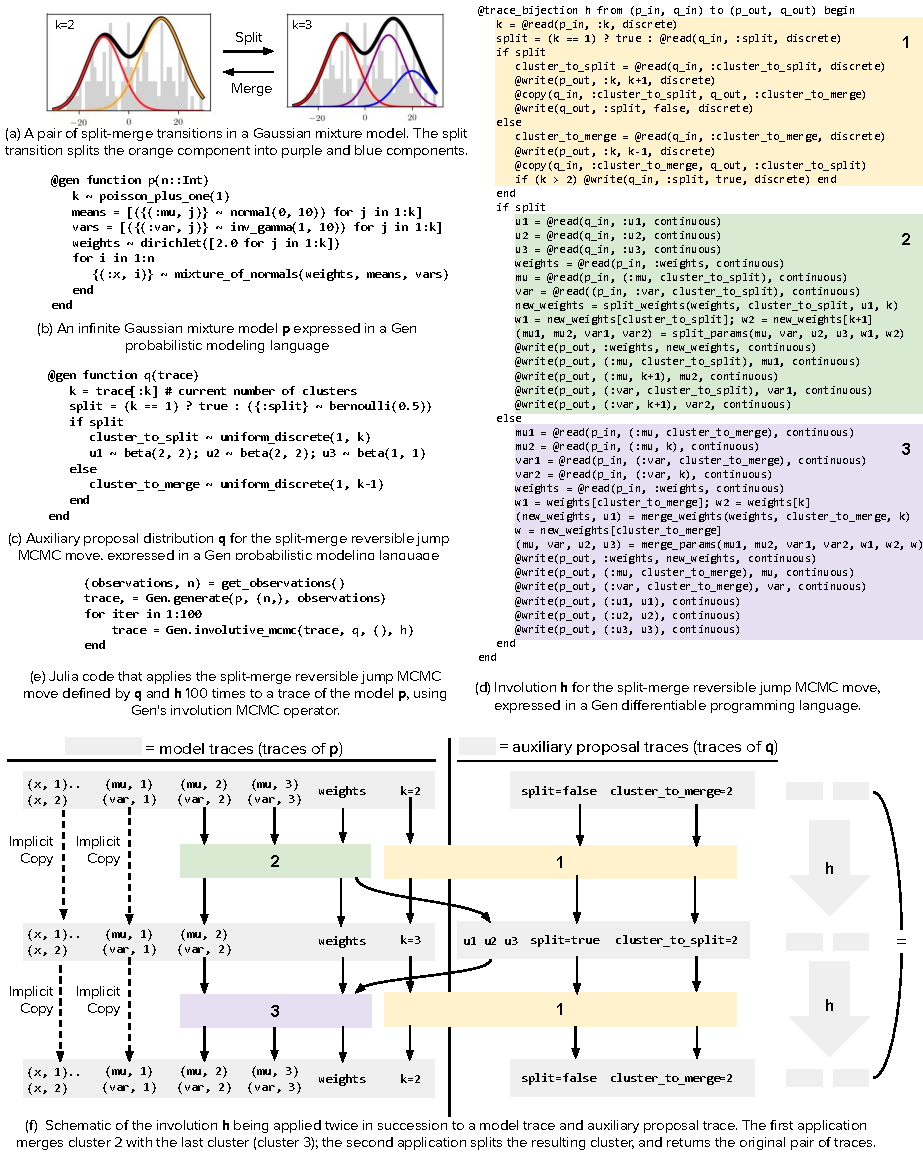
\includegraphics[width=\textwidth]{figures/mixture.pdf}
    \caption{
Example of reversible jump MCMC~\citep{green1995reversible} implemented using involutive MCMC in Gen.
The example implements a `split-merge move' in a infinite Gaussian mixture model~\citep{richardson1997bayesian} using three Gen programs:
(1) a probabilistic program $\mathtt{p}$ encoding the generative model (shown in b),
(2) a probabilistic program $\mathtt{q}$ encoding an auxiliary probability distribution (shown in c),
and (3) a differentiable program $\mathtt{h}$ that encodes an involution on the space of pairs of traces of $\mathtt{p}$ and $\mathtt{q}$ (shown in d).
Gen's involutive MCMC operator (shown in e) automatically computes the acceptance probability.
}
    \label{fig:mixture}
\end{figure*}

\begin{figure*}[ht]
    \centering
    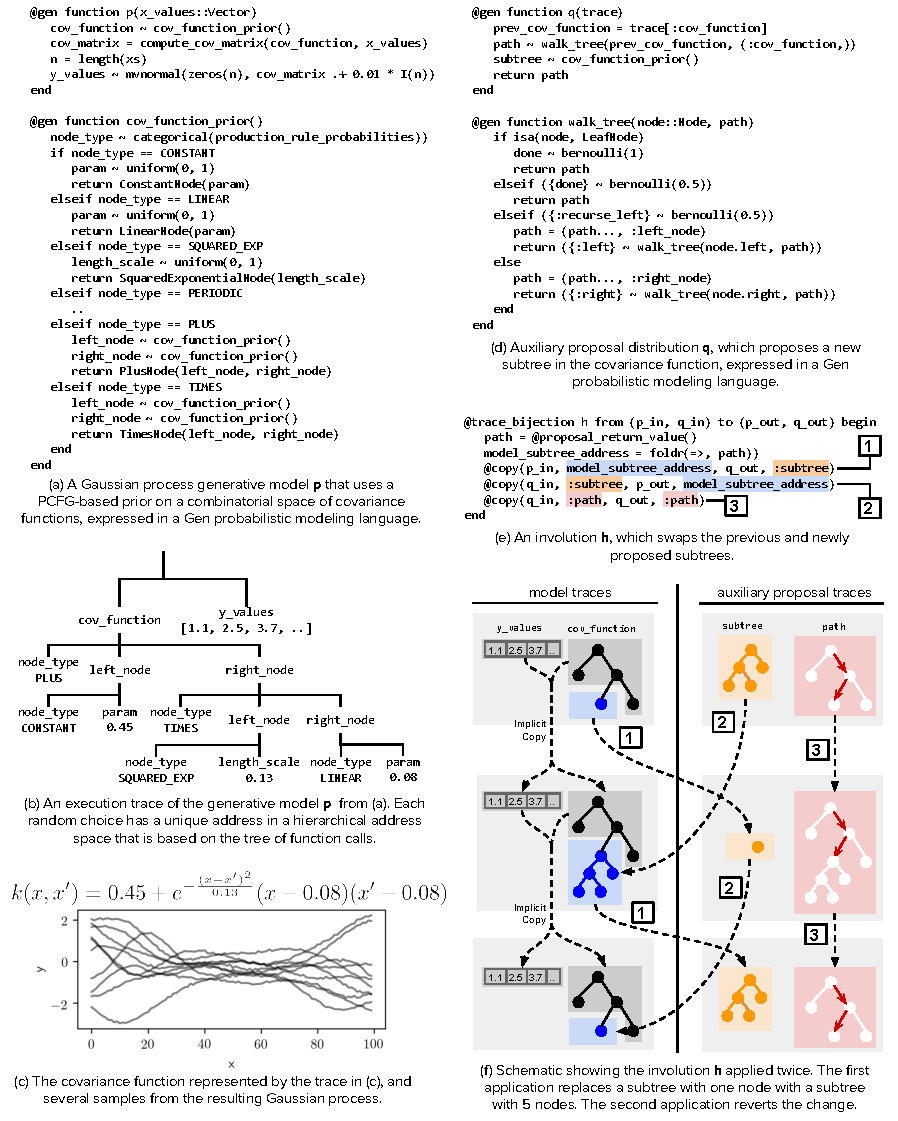
\includegraphics[width=\textwidth]{figures/structure-learning.pdf}
    \caption{
A mixture kernel implemented using involutive MCMC in Gen, applied to infer the covariance function of a Gaussian process.
The prior on covariance functions is based on a probabilistic context-free grammar.
Each component kernel in the mixture replaces a subtree of the covariance function parse tree with a new subtree.
The mixture kernel chooses a random subtree to replace via a random walk on the parse tree.
The mixture kernel is composed from three Gen programs:
(1) a probabilistic program $\mathtt{p}$ encoding the generative model (shown in a),
(2) a probabilistic program $\mathtt{q}$ encoding an auxiliary probability distribution (shown in b), and
(3) a differentiable program $\mathtt{h}$ that encodes an involution (shown in d).
}
    \label{fig:structure-learning}
\end{figure*}



\section{INVOLUTIVE MCMC ON GENERAL STATE SPACES} % on traces ??

Involutive MCMC is a general framework for constructing MCMC kernels that are stationary
for a target probability measure $p$. Informally, the algorithm works as follows: starting at some state $x$, we first sample
an auxiliary variable $y \sim q_x$ from a state-dependent auxiliary distribution. We then apply an \textit{involution} $f$ to the pair $(x, y)$ to obtain $(x', y')$. 
Finally, we computes an acceptance probability $\alpha$ and either accept $x'$ as the new state, or reject it and repeat the previous state $x$.
Different choices of $q$ and $f$ recover many algorithms from the literature~\citep{imcmc}.

In this section, we derive the involutive MCMC algorithm for models $p$ and auxiliary kernels
$q$ defined over general state spaces.
By emphasizing general state spaces, we intend to clarify
a potential point of confusion regarding the involutive MCMC algorithm: as presented by
\citet{imcmc},
the acceptance probability $\alpha$ depends on the Jacobian of the involution $f$, but
it is not immediately clear how to define this Jacobian when $f$ may operate on samples
from arbitrary measurable spaces, rather than on vectors in $\mathbb{R}^n$. Our 
reformulation of the algorithm below is general enough to handle arbitrary model and auxiliary
distributions, and precise enough to enable automation via probabilistic and differentiable
programming: the rest of this paper uses it to develop a technique for deriving efficient implementations
of involutive MCMC algorithms automatically, 
given only declarative specifications of $p$, $q$, and $f$.

\subsection{Distributions on Dictionaries}

Instead of vectors of real numbers, we consider in this section distributions over 
\textit{finite dictionaries} that map (possibly random) keys to (possibly random) values. 
Dictionaries include vectors as a special case (a vector $\mathbf{x} \in \mathbb{R}^n$ can
be represented as a dictionary mapping the keys $1, \dots, n$ to the values $x_1, \dots, x_n$),
but are in general more flexible: different keys can hold values of different types, and we
can also consider distributions in which the set of keys is itself random, useful for model
selection problems and structure uncertainty more generally.

\textbf{The space of finite dictionaries.}
We fix a countably infinite set $\mathcal{A}$ of possible keys, such that each key $a$ is either \emph{discrete} ($a \in \mathcal{I}$) or \emph{continuous} ($a \in \mathcal{J}$), where $\mathcal{A} = \mathcal{I} \cup \mathcal{J}$.\footnote{
It is straightforward to assign a general measure space to each address, but this is not necessary for our purposes.}
Let $V_a$ denote the set of possible values for key $a$, where $V_a$ is a countable set for each discrete key, and where $V_a = \mathbb{R}^{d_a}$ for each continuous key for some $d_a$.
Given a set of keys $A$, let $V_A = \times_{a \in A} V_a$ denote the set of \textit{assignments} of values to each key.
Then the set of all finite dictionaries is $\mathcal{D} := \bigcup_{A \subset \mathcal{A}, |A| < \infty} \{(A, \mathbf{x}) \mid \mathbf{x} \in V_A\}$. That is, a dictionary specifies 
a finite set of keys $A \subset \mathcal{A}$ at which it has values, and an assignment $\mathbf{x}$ of values $x_a$ for each.

\textbf{A measure space of finite dictionaries.}
We associate a measure $\mu_a$ on $V_a$ for each key---the counting measure for each discrete key and the Lebesgue-measure on $\mathbf{R}^{d_a}$ for each continuous key.
For each finite set of keys $A$, we make $V_A$ a measure space using the standard product $\sigma$-algebra $\Sigma_A = \otimes_{a \in A} \Sigma_a$ and the product measure $\mu_A = \times_{a \in A} \mu_a$.
We equip $\mathcal{D}$ with the $\sigma$-algebra $\Sigma_{\mathcal{D}} := \{\bigcup_{A \subset \mathcal{A}, |A| < \infty} \{(A, \mathbf{x}) \mid \mathbf{x} \in B_A\} \mid B_A \in \Sigma_A \, \text{for each finite } A \subset \mathcal{A}\}$ to obtain a measurable space
of dictionaries.
A reference measure $\mu_\mathcal{D}$ on this space can be constructed using the product measures $\mu_A$: we set $\mu(B) := \sum_{A \in \mathcal{A}, |A| < \infty} \mu_A(\{\mathbf{x} \mid (A, \mathbf{x}) \in B\})$.

\textbf{Notation for dictionaries.} Given a dictionary $d = (A, \mathbf{x})$, we write $A_d$ for $A$ and $d[a]$ for the value $x_a$ associated with a key $a \in A$.
We also denote specific dictionaries using notation $\{k_1 \mapsto v_1, k_2 \mapsto v_2, \ldots\}$.
For example, the dictionary $(A, \mathbf{x})$ with $A = \{1, \mathtt{"foo"}\}$ and $x_1 = 0.123$ and $x_{\mathtt{"foo"}} = 5$ is denoted 
$\{1 \mapsto 0.123, \mathtt{"foo"} \mapsto 5\}$.

\textbf{Probability distributions on finite dictionaries.} 
When all keys are discrete, a probability distribution on dictionaries is defined by a $p$ is a probability mass function $p : \mathcal{D} \to [0, 1]$ that assigns a probability $p(m)$ to each dictionary $m \in \mathcal{P}$ such that $\sum_{x \in \mathcal{D}} p(m) = 1$.
More generally a probability distribution in dictionaries is defined by a probability density $p : \mathcal{D} \rightarrow [0, \infty)$ such that $\int p(m) \mu_\mathcal{D}(\text{d}m) = 1$. We now give several examples
to build intuition.

% TODO keys vs addresses

% TODO how to notate dictionaries -- 'm' or 'd' or 'x' or 't'?

\textit{Gaussian mixture model with unknown number of components.} Consider a generative model of univariate data points $y_1, \dots, y_n$ from a Gaussian mixture with an unknown number of components $k$, each with unknown mean $m_i$ and variance $s_i$. If we place a Gaussian prior on $m_i$, an inverse Gamma prior on $s_i$, and a Poisson prior on $k$, the resulting density is
%
\begin{align*}
p(d) =
\begin{array}{l}
p_{\mathrm{poisson}(3)}(d[\mathtt{k}]) \cdot\\
\prod_{i=1}^{d[\mathtt{k}]} p_{\mathrm{normal}(0, 1)}(d[\mathtt{m}_i]) \cdot\\
\prod_{i=1}^{d[\mathtt{k}]} p_{\mathrm{inversegamma}(1, 10)}(d[\mathtt{s}_i]) \cdot\\
\prod_{i=1}^n  \frac{1}{d[\mathtt{k}]} \sum_{j=1}^{d[\mathtt{k}]} \cdot p_{\mathrm{normal}(d[\mathtt{m}_j], d[\mathtt{s}_i])}(d[\mathtt{y}_i])
\end{array}
\end{align*}
%
when $A_d$ is of the form $\{\texttt{k}, \texttt{y}_\texttt{1}, \dots, \texttt{y}_\texttt{n}\} \cup \{\texttt{m}_i \mid 1 \leq i \leq d[\texttt{k}]\} \cup \{\texttt{s}_i \mid 1 \leq i \leq d[\texttt{k}]\}$, and 0 otherwise. In this case, we have $V_\texttt{k} = \mathbb{N}$ with the counting measure for $\mu_\texttt{k}$, and for all other addresses $a \in \mathcal{A}$, $V_a = \mathbb{R}$ with the Lebesgue measure for $\mu_a$.

\textit{Polynomial regression.} 

TODO

\textbf{Conditional distributions via disintegration.} Consider a probability density $p$ on the space $\mathcal{D}$ of dictionaries. 
%For a set of keys $A \subset \mathcal{A}$, let $p(A) := \int 1[A_m = A] p(m) \mu_\mathcal{D}(\text{d}m)$, the probability under $p$ of a dictionary with exactly the key set $A$. 
We say a key $a \in \mathcal{A}$ \textit{almost always appears} if $\int \mathbf{1}[a \in A_m] p(m) \mu_\mathcal{D}(\text{d}m) = 1$. Suppose $B$ is a set of keys that almost always appear for $p$, and that $b = (B, \mathbf{b})$ is a dictionary with keys $B$. Furthermore, let $(A_m, \mathbf{m}) \oplus (A_n, \mathbf{n}) := (A_m \cup A_n, \mathbf{m} \times \mathbf{n})$ be the \textit{merge} of two dictionaries $m$ and $n$ defined on disjoint key sets $A_m$ and $A_n$. Then we can define the conditional density $p(d \mid b) := \mathbf{1}[A_d \cap B = \emptyset] \frac{p(d \oplus b)}{\int_{\{m \mid A_m \cap B = \emptyset\}} p(m \oplus b) \mu_\mathcal{D}(\text{d}m)}$ when the denominator is finite. If the reference measure $\mu_a$ associated with each key $a \in B$ is discrete (e.g., the counting measure), then this definition corresponds to the ordinary notion of conditioning on an event (namely, the event that a sample from $p$ agrees with the dictionary $b$ on all addresses in $B$). When this is not the case, it corresponds to a more general measure-theoretic notion called disintegration~\citep{disintegration1997}. 

\subsection{Involutive MCMC}

Let $(X, \Sigma_P, \mu_P)$ and $(Y, \Sigma_Q, \mu_Q)$ denote two general measure spaces with $\sigma$-finite $\mu_P$ and $\mu_Q$. 
Involutive MCMC (Algorithm~\ref{alg:involutive-mcmc}) implements a transition kernel that is invariant for a \textit{model distribution} given by $p : X \to [0, \infty)$, a probability density over $X$ with respect to $\mu_P$. Each iteration, the algorithm first samples auxiliary variables $y \in Y$ from an \emph{auxiliary distribution} $q_x$ based on the model's current state $x$: for each $x \in X$ such that $p(x) > 0$, $q_x : Y \to [0, \infty)$ is a probability density with respect to $\mu_Q$.
% We call $p$ the \emph{model density} and we call $q_x$ \emph{auxiliary densities}.

The resulting pair $(x, y)$ of the current model state and the newly sampled auxiliary state will be an element of the joint space $Z := \{(x, y) \in X \times Y \mid p(x) q_x(y) > 0 \}$. We can equip $Z$ with the $\sigma$-algebra 
$\Sigma := \{A \cap Z \mid A \in \Sigma_P \otimes \Sigma_Q\}$ (assuming $Z$ is a $\mu_P \times \mu_Q$-measurable set), and a reference measure $\mu(A) := (\mu_P \times \mu_Q)(A)$. 
%Let $\pi(x, y) := p(x) q_x(y)$ and $Z := \{(x, y) \in X \times Y : \pi(x, y) > 0 \}$.
%Suppose that $Z \in \Sigma_P \otimes \Sigma_Q$ ($Z$ is a $\mu_P \times \mu_Q$-measurable set).
%Then $\Sigma := \{A \in \Sigma_P \otimes \Sigma_Q : A \subseteq Z\}$ is a $\sigma$-algebra on $Z$ and $\mu : \Sigma \to [0, \infty)$ with $\mu(A) := (\mu_P \times \mu_Q)(A)$ is a $\sigma$-finite measure on measurable space $(Z, \Sigma)$.

Let $f : Z \to Z$ denote an involution ($f^{-1} = f$) such that the pushforward of $\mu$ under $f$, denoted $\mu \circ f^{-1}$, is absolutely continuous with respect to $\mu$, with Radon-Nikodym derivative $d (\mu \circ f^{-1}) / d\mu : Z \to [0, \infty)$. Involutive MCMC runs $f$ on $(x, y)$ to obtain $(x', y')$, then computes an acceptance probability $\alpha$.
With probability $\alpha$, the new state $x'$ is returned; otherwise, the previous state $x$ is repeated.
%Let $y \sim q_x(\cdot)$ denote a random sample from the measure defined by $A \mapsto \int_A q_x(y) \mu_Q(dy)$ for $A \in \Sigma_Q$.

\begin{theorem}[Involutive MCMC is stationary]
Involutive MCMC defines a probability kernel $k$ on $X$ that is stationary with respect to the model probability distribution.
That is, $\int_X k_x(B) p(x) d\mu_X(dx) = \int_B p(x) d\mu_X(dx)$ for all $B \in \Sigma_X$.
\end{theorem}
\begin{proof}
The proof is presented in stages in the appendix (see Section~\ref{sec:involution-detailed-balance}, Section~\ref{sec:involution-is-stationary}, and Section~\ref{sec:involutive-mcmc-is-stationary}).
\end{proof}


\subsection{Involutive MCMC with Dictionaries}

The general measure-theoretic formulation of involutive MCMC in Algorithm~\ref{alg:involutive-mcmc} does not specify how to compute the Radon-Nikodym derivative that is required for the acceptance probability.
When the algorithm is specialized for state spaces consisting of dictionaries, the acceptance probability simplifies and can be computed from standard Jacobian and probability density computations.
Because dictionaries are flexible objects, the algorithm remains quite general.

Suppose that the model distribution $p$ and auxiliary distributions $q_x$ are all probability distributions on dictionaries.
Then, $X$ and $Y$ are both sets of dictionaries, and the joint space $Z$ is a set of pairs $(x, y)$ of dictionaries with keys $\mathcal{A}$, so that $Z = X \times Y \subseteq \mathcal{D} \times \mathcal{D}$.
%And suppose that there exists an involution $f : Z \to Z$ such that (i) 
Suppose there is a countable partition of $Z$ into $\{Z_e : e \in E\}$ such that across each $Z_e$ the sets of keys $A_x$ and $A_y$ and the values $x_a$ and $y_a$ for all discrete keys $a$ are both constant (so that each set $Z_e$ is isomorphic to a Euclidean space of assignments to the continuous keys in the two dictionaries).
Suppose there is an involution $g : E \to E$ between elements of the partition (a function with $g = g^{-1}$), and a family of continuously differentiable bijections $h_{e} : Z_e \to Z_{g(e)}$ for each $e$ with $h_{e} = h_{g(e)}^{-1}$.
Let $e(z) \in E$ denote the element of the partition for an alement $z \in Z$.
Then, $f : Z \to Z$ given by $f(z) := h_{e(z)}(z)$ is an involution:
\begin{equation}
f(f(z)) = h_{e(f(z))}(h_{e(z)}(z)) = h_{g(e(z))}(h_{e(z)}(z)) = z
\end{equation}
Let $|J h_e|(z)$ denote the absolute value of the Jacobian (determinant) of $h_e$, evaluated at $z$.
Then, the acceptance probability simplifies to:
\begin{equation}
\alpha(x, y) = \frac{p(x') q_{x'}(y')}{p(x) q_{x}(y)} \cdot |J h_e|(z)
\end{equation}
Section~\ref{sec:radon-nikodym-special-case} of the appendix for details.

\begin{algorithm}[h]
\begin{algorithmic}
\Procedure{involutive-mcmc}{$p$, $q$, $f$, $x$}
    \State $y \sim q_x(\cdot)$ \Comment{Sample auxiliary state}
    \State $(x', y') \gets f(x, y)$ \Comment{Apply involution}
    \State $\alpha \gets
        \displaystyle \frac{p(x') q_{x'}(y')}{p(x) q_{x}(y)} \cdot \left( \frac{d (\mu \circ f^{-1})}{d \mu} (x, y)\right)$
    \State $r \sim \mathrm{Uniform}(0, 1)$
    \State \algorithmicif \, $r \le \alpha$ \algorithmicthen \, \Return $x'$ \algorithmicelse \, \Return $x$ 
\EndProcedure
\end{algorithmic}
\caption{Involutive MCMC}
\label{alg:involutive-mcmc}
\end{algorithm}


%\section{AUTOMATING INVOLUTIVE MCMC} \label{sec:involutive-mcmc}

%Involutive MCMC (Algorithm~\ref{alg:involutive-mcmc}) defines a transition kernel that is stationary for a probabilistic model $p$, based on an auxiliary probability kernel $q$ and a deterministic involution $f$. Different choices of $q$ and $f$ recover instances of classic algorithms from the literature (e.g., Reversible-Jump MCMC~\citep{green}, TODO: others). This section briefly reviews involutive MCMC and gives a general measure-theoretic formulation of the algorithm on arbitrary state-spaces. In the following sections, we will describe how the implementations of involutive MCMC algorithms can be automated using probabilistic and differentiable programming.

\section{AUTOMATING INVOLUTIVE MCMC} \label{sec:automating}

% TODO add the algorithm box involving traces..

\begin{algorithm*}[h]
\begin{algorithmic}
\Procedure{auto-involutive-mcmc}{$\mathcal{P}$, $\mathcal{Q}$, $\mathcal{F}$, $x$}
    \State $(y, \log w_2) \gets \textproc{trace-and-score}(\mathcal{Q}_x)$ \Comment{Sample $y \sim q_x(\cdot)$ and compute log-density $\log q_x(y)$}
    \State $(x', y', \log D) \gets \textproc{run-involution}(\mathcal{F}, (x, y))$ \Comment{Compute $(x', y') = f(x, y)$, log Radon-Nikodym deriv. $\log D$}
    \State $\log w_1 \gets \textproc{score}(\mathcal{P}, x)$ \Comment{Compute log-density $\log p(x)$}
    \State $\log w_3 \gets \textproc{score}(\mathcal{P}, x')$ \Comment{Compute log-density $\log p(x')$}
    \State $\log w_4 \gets \textproc{score}(\mathcal{Q}_{x'}, y')$ \Comment{Compute log-density $\log q_{x'}(y')$}
    \State $\alpha \gets \min\{1, \exp(\log w_3 - \log w_1 + \log w_4 - \log w_2 + \log J)\}$ \Comment{Compute acceptance probability}
    \State \textbf{with probability} \,$\alpha$ \,\Return $x'$ \algorithmicelse \, \Return $x$ 
\EndProcedure\\

\begin{minipage}[t]{0.5\linewidth}
\Procedure{trace-and-score}{$\mathcal{P}$}
   \State $\log w \gets 0$
   \State $x \gets \{\}$
   \execute[$\mathcal{P}$], but with $\mathtt{"a \sim d"} \equiv$ (
        \State \hspace{5mm} 1. set $v \sim d$
        \State \hspace{5mm} 2. set $x[a] \gets v$
        \State \hspace{5mm} 3. set $\log w \gets \log w + \textproc{logpdf}(d, v)$
        \State \hspace{5mm} 4. evaluate to $v$)
    \END
   \State \Return $(x, \log w)$
\EndProcedure
\end{minipage}%
\begin{minipage}[t]{0.5\linewidth}
\Procedure{score}{$\mathcal{P}$, $x$}
   \State $\log w \gets 0$
   \execute[$\mathcal{P}$], but with $\mathtt{"a \sim d"} \equiv$ (
        \State \hspace{5mm} 1. set $v \gets x[a]$
        \State \hspace{5mm} 2. set $\log w \gets \log w + \textproc{logpdf}(d, v)$
        \State \hspace{5mm} 3. evaluate to $v$)
    \END
   \State \Return $\log w$
\EndProcedure
\end{minipage}\\

\Procedure{run-involution}{$\mathcal{F}$, $(x, y)$}
% TODO would be much simpler to describe if we didn't have to separate out x and y..
    \LineComment{Run the involution, and keep track of continuous addresses}
    \State $x' \gets \{\}$ \Comment{Initialize empty output dictionary}
    \execute[$\mathcal{F}$], but with
        \State $\mathtt{"write\_cont}(a, v)\mathtt{"} \equiv$ (1. set $x'[a] \gets v$ and 2. set $W \gets W \cup \{a\}$)
        \State $\mathtt{"read\_cont}(a)\mathtt{"} \equiv$ (1. set $R \gets R \cup \{a\}$ and 2. evaluate to $x[a]$)
        \State $\mathtt{"copy}(a_1, a_2)\mathtt{"} \equiv$ (1. set $x'[a_2] \gets x[a_1]$ and 2. set $C \gets C \cup \{a_2\}$)
    \END
    \LineComment{Use automatic differentiation to compute Jacobian, skipping copied addresses}
    \For{$i$ in $1, \ldots, |W \setminus C|$}
        \State $J[i,:] \gets \nabla_{x_{R \setminus C}} \left( h_{e(x, y)}[(W \setminus C)_i] \right)$ \Comment{Gradient of $x'[(W \setminus C)_i]$ w.r.t. non-copied continuous inputs}
    \EndFor
    \State \Return $(x', \log |\det(J)|)$
\EndProcedure

\end{algorithmic}
\caption{Automated Involutive MCMC}
\label{alg:auto-involutive-mcmc}
\end{algorithm*}

Involutive MCMC is a general framework that can be used to develop diverse MCMC algorithms
for models over arbitrary state spaces. We wish to \textit{automate} the implementation
details for involutive MCMC algorithms, given only a specification of the model $p$, the
auxiliary distribution $q$, and the involution $f$.
To do so, we require a representation for the distributions $p$ and $q$ that is flexible
enough to represent the full variety of models and auxiliary distributions of interest to
practitioners. The representation must support density evaluation and sampling. It is also desirable that the representation be \textit{structured}: the more
information available to us (e.g., about the decomposition of a distribution's state space into 
individual univariate and multivariate random variables, or about conditional independence relationships in a model),
the easier it will be for the implementation to exploit this structure automatically by using
more efficient data structures and low-level manipulations.

\subsection{Trace-Based Probabilistic Programming}

\textit{Probabilistic programs} are flexible and structured representations for  probability distributions. Unlike densities (but like Bayesian networks), probabilistic programs can be efficiently sampled and contain explicitly represented information
about some conditional independence relationships in a model. 
But unlike Bayesian networks, they do not assume a fixed number of random variables, state space dimension, or dependency structure.

At the most basic level, a probabilistic program is a program that makes random choices. 
Any such program induces a probability distribution over its possible \textit{execution traces}, records of each random choice it makes.
If each random choice is associated with a unique \textit{address} from a countable set
of addresses $\mathcal{A}$, 
then these traces can be viewed as finite dictionaries, mapping the address of each random choice to its value. 
The distribution induced by a probabilistic program over
its execution traces can thus be understood as a measure on the space $(\mathcal{D}, \Sigma_\mathcal{D}, \mu_\mathcal{D})$ introduced in the previous section. Furthermore, densities of trace distributions with respect to $\mu_\mathcal{D}$ are typically easy to compute.

In this section, we introduce the Gen language~\citep{gen-pldi} for probabilistic programs, and present a technique for automating the implementation of involutive MCMC algorithms when the model $p$ and auxiliary distribution $q_x$ are both represented as
Gen programs. 

\subsubsection{A Language for Probabilistic Programs with Traces}

The Gen probabilistic programming language augments the syntax of Julia~\citep{julia}
with a single new construct, the \texttt{\{a\} $\sim$ d} expression, for making a \textit{named} random choice. An execution trace of a Gen probabilistic program can be sampled by running the program according to Julia's usual semantics, and upon encountering an expression of the form \texttt{\{a\} $\sim$ d}, (i) evaluating the \textit{address expression} \texttt{a} to obtain an address $a \in \mathcal{A}$; (ii) evaluating the \textit{distribution expression} $d$ to obtain a distribution $d$ over the measurable space $V_a$; (iii) sampling a value $x_a \sim d$ and adding the mapping $\{a \mapsto x_a\}$ to a dictionary called the program trace; and (iv) returning the sampled value $x_a$ to the program, to continue execution. When execution terminates, the program trace has accumulated a mapping for each random choice encountered during the program's execution.

As a concrete example, consider Figure~\ref{fig:mixture}a, which defines a Gen program for a Gaussian mixture model with an unknown number of components. The program \texttt{p} accepts as input an integer \texttt{n}, a number of data points. Each $\texttt{n}$ defines
a distinct distribution over dictionaries.

The first line of the program samples a number of mixture components from a Poisson prior using the address \texttt{:k}. (This line could also be written \texttt{k = \{:k\} $\sim$ poisson\_plus\_one(1)}: the \textit{address} is the symbol \texttt{:k}, and the result of the choice is assigned to a Julia variable called \texttt{k}. Because this is a common pattern, Gen provides the syntactic sugar \texttt{x $\sim$ d} as shorthand for \texttt{x = \{:x\} $\sim$ d}.) The program then samples \texttt{k} means and \texttt{k} variances from Gaussian and inverse Gamma priors, respectively. Each of these 2\texttt{k} random choices has its own address, determined by the address expression preceding it. For example, the mean for the fourth mixture component (if \texttt{k} $\geq 4$) has address \texttt{(:mu, 4)}. The mixture weights are then sampled at the address \texttt{:weights} from a Dirichlet distribution, and $\texttt{n}$ data points are sampled at addresses \texttt{(:x, 1)}, \dots, \texttt{(:x, n)}. The random choice at address $\mathtt{:}\mathtt{k}$ is discrete with $V_{\texttt{:k}} = \integers_{\ge 1}$, and the other random choices are continuous. 
Overall, the program defines a distribution over traces with the following density over traces $(A, \mathbf{x})$ with respect to $\mu_\mathcal{D}$:
\begin{align*}
p(n)((A, \mathbf{x})) =
\begin{array}{l}
p_{\mathrm{poisson}(1)}(x_{\mathtt{:}\mathtt{k}}-1) \cdot\\
\prod_{i=1}^{x_{\mathtt{:}\mathtt{k}}} p_{\mathrm{normal}(0, 10)}(x_{(\mathtt{:}\mathtt{mu}, i)}) \cdot\\
\prod_{i=1}^{x_{\mathtt{:}\mathtt{k}}} p_{\mathrm{inversegamma}(1, 10)}(x_{(\mathtt{:}\mathtt{var}, i)}) \cdot\\
p_{\mathrm{dirichlet}(2.0,\dots,2.0)}(x_{\mathtt{:}\mathtt{weights}})\cdot\\
\prod_{i=1}^n \sum_{j=1}^{x_{\mathtt{:}\mathtt{k}}} x_{\mathtt{:}\mathtt{weights}}[j] \cdot\\
\;\;\;\;\;\;\;\;\;\;\;\;\;\;\;\;\;\; p_{\mathrm{normal}(x_{\mathtt{(:mu, j)}}, x_{(\mathtt{:}\mathtt{var}, j)})}(x_{(\mathtt{:}\mathtt{x}, i)})
\end{array}
\end{align*}
when $A$ contains exactly the addresses $\mathtt{:}\mathtt{k}, \mathtt{:}\mathtt{weights}, (\mathtt{:}\mathtt{x}, i)$ for $i = 1, \dots, n$, and $(\mathtt{:}\mathtt{mu}, j)$ and $(\mathtt{:}\mathtt{var}, j)$ for $j = 1, \dots, x_{\mathtt{:}\mathtt{k}}$; otherwise, the density is 0.

% where $m(t, i) := \sum_{j=0}^{x[\mathtt{:}\mathtt{degree}]} \mathtt{xcoords}[i]^j \cdot x[(\mathtt{"c"}, j)]$, and where $p_{\mathrm{geometric}(r)}$, $p_{\mathrm{inversegamma}(\alpha, \beta)}$, and $p_{\mathrm{normal}(\mu, \sigma)}$ are density functions for geometric, inverse gamma, and normal distributions, respectively.




% The addresses used by this generative function are:
% \[
% \mathcal{A} := \begin{array}{c}
% \{\mathtt{:}\mathtt{noise}, \mathtt{:}\mathtt{degree}\} \bigcup
% \{(\mathtt{"c"}, i) : i \in \integers_{\ge 0}\} \bigcup\\
% \{(\mathtt{"y"}, i) : i \in \integers_{> 0}\}
% \end{array}
% \]
% (Note that $\mathcal{A}$ could contain additional addresses that the program never samples.)
% The random choice at address $\mathtt{:}\mathtt{degree}$ is discrete with $V_a = \integers_{\ge 0}$ and the other random choices are continuous.
% The address $\mathtt{:}\mathtt{noise}$ has $V_a = \reals_{> 0}$ and $(\mathtt{"c"}, i)$ and $(\mathtt{"y"}, i)$ have $V_a = \reals$, and at all of these continuous addresses, we use the Lebesgue measure for $\mu_a$. % TODO double-check this
% The density with respect to the reference measure $\mu$ is then:
% \begin{align*}
% p(x) =
% \begin{array}{l}
% p_{\mathrm{geometric}(0.5)}(x[\mathtt{:}\mathtt{degree}]) \cdot\\
% p_{\mathrm{inversegamma}(1, 1)}(x[\mathtt{:}\mathtt{noise}]) \cdot\\
% \prod_{0=1}^{x[\mathtt{:}\mathtt{degree}]} p_{\mathrm{normal}(0,1)}(x[(\mathtt{"c"}, i)])\cdot\\
% \prod_{i=1}^n p_{\mathrm{normal}(m(t, i), 0.1 + x[\mathtt{noise}])}(x[(\mathtt{"y"}, i)])
% \end{array}
% \end{align*}
% where $m(t, i) := \sum_{j=0}^{x[\mathtt{:}\mathtt{degree}]} \mathtt{xcoords}[i]^j \cdot x[(\mathtt{"c"}, j)]$, and where $p_{\mathrm{geometric}(r)}$, $p_{\mathrm{inversegamma}(\alpha, \beta)}$, and $p_{\mathrm{normal}(\mu, \sigma)}$ are density functions for geometric, inverse gamma, and normal distributions, respectively.







% In our framework, a probabilistic program defines a probability distribution on finite maps (dictionaries) that map the names of random choices (their \emph{addresses}) to values.
% % TODO trace terminology
% Following standard terminology~\citep{?}, we call these dictionaries \emph{traces} because they are often sampled by running a probabilistic program, and `tracing' the execution of the program by recording the value of each random choice encountered.
% We now make the concept of a trace more concrete using code in a probabilistic programming language.

% The probabilistic programming language used in this paper is 
% the dynamic modeling language in the Gen probabilistic programming system~\citep{gen-pldi}.
% The language is embedded in the general-purpose Julia programming language~\citep{julia}.
% Julia functions can be turned into Gen probabilistic programs by tagging
% each random choice with an explicit address in the code, 
% as part of a \emph{random-choice expression} of the following form:
% \noindent
% \begin{center}
% \begin{tabular}{c}
% {\begin{lstlisting}[basicstyle=\small\ttfamily]
% {<address>} ~ <distribution>
% \end{lstlisting}}
% \end{tabular}
% \end{center}
% The left-hand side of the expression (green) specifies the address of the choice, and the right-hand side specifies the probability distribution to be sampled from.
% For example, the following expression samples a non-negative integer from a geometric distribution and the value gets recorded in the trace at the address \texttt{"a"}:
% \noindent
% \begin{center}
% \begin{tabular}{c}
% {\begin{lstlisting}[basicstyle=\small\ttfamily]
% {"a"} ~ geometric(0.5)
% \end{lstlisting}}
% \end{tabular}
% \end{center}
% In addition to being recorded in the trace, the sampled value is returned to the running program.
% That is, the random choice expression evaluates to the sampled value.
% For example, the expression below samples the random variable \texttt{"a"} and multiplies it by 2,
% yielding an even non-negative integer:
% \noindent
% \begin{center}
% \begin{tabular}{c}
% {\begin{lstlisting}[basicstyle=\small\ttfamily]
% ({"a"} ~ geometric(0.5)) * 2
% \end{lstlisting}}
% \end{tabular}
% \end{center}
% A probabilistic program will typically combine multiple random choice expressions. For example,
% the following code samples a random choice at address \texttt{"a"}, assigns it to the Julia variable
% \texttt{a}, and then samples a Bernoulli random variable at address \texttt{"b"} with a parameter
% that depends on \texttt{a}:
% \noindent
% \begin{center}
% \begin{tabular}{c}
% {\begin{lstlisting}[basicstyle=\small\ttfamily]
% a = ({"a"} ~ geometric(0.5))
% {"b"} ~ bernoulli(a / (a + 1))
% \end{lstlisting}}
% \end{tabular}
% \end{center}
% This probabilistic program has an unbounded (countably infinite) number of possible traces it could produce.
% One possible trace samples the value 1 at $\texttt{"a"}$ and the Boolean value $\false$ at \texttt{"b"}, and we denote this trace by $\{\mathtt{"a"} \mapsto 1, \mathtt{"b"} \mapsto \false\}$.
% Note that the Julia variable to which the first choice is assigned (\texttt{a}) happens to be the same as the address (\texttt{"a"}).
% This is not required, and often the random choice has no corresponding Julia variable in the program, as in the second random choice with address \texttt{"b"}.
% But to reduce unnecessary typing, the following optional syntactic sugar will simultaneously assign the value to the program variable $\mathtt{a}$ and record it at trace address $\mathtt{"a"}$.\footnote{
% More precisely, the address is the Julia symbol (interned string) \texttt{a}, constructed with Julia syntax \texttt{:a}.}
% \noindent
% \begin{center}
% \begin{tabular}{c}
% {\begin{lstlisting}[basicstyle=\small\ttfamily]
% a ~ geometric(0.5)
% \end{lstlisting}}
% \end{tabular}
% \end{center}

% What gives probabilistic programs much of their expressive power is that they can make use of familiar control flow constructs, like loops and if statements, and this control flow can both depend on random choices and influence which random choices are made downstream. Consider the following program implementing a geometric
% distribution as the result of iterated Bernoulli draws:
% \noindent
% \begin{center}
% \begin{tabular}{c}
% {\begin{lstlisting}[basicstyle=\small\ttfamily]
% i = 1
% while ({i} ~ bernoulli(0.5))
%     i = i + 1
% end
% \end{lstlisting}}
% \end{tabular}
% \end{center}
% Note that each Bernoulli flip uses a different address (the number \texttt{i} increases at each iteration). For the probabilistic program to be valid, we require that every address is used at most once within every possible execution.

% For probabilistic programs that sample from discrete probability distributions like those used above, the meaning of the program is a probability mass function $p$ that assigns a probability to every possible trace.
% For example, for the program with the \texttt{while} loop above, the distribution is:
% \[
% \begin{array}{c|c}
%     x & p(x)\\
%     \hline
%     \{1 \mapsto \false\} & 0.5\\
%     \{1 \mapsto \true, 2 \mapsto \false\} & 0.5^2\\
%     \{1 \mapsto \true, 2 \mapsto \true, 3 \mapsto \false\} & 0.5^3\\
%     .. & ..
% \end{array}
% \]
% We assume that probabilistic programs halt with probability $1$, meaning that the sum of probabilities over all (finite) traces is one.
% Note that traces are always finite, but there may be an infinite number of possible traces, as in the previous example.

% In order to construct more complex distributions, we wrap probabilistic programs in functions, called
% `generative functions' in Gen.
% These functions can then be invoked by other functions, including recursively, which allows programs encode probability distributions on more complex and combinatorial objects.
% When invoking such a function, we give an \emph{address namespace} under which every random choice made in that function should be recorded.
% This helps prevent addresses of choices defined in different functions from colliding.
% The syntax for calling a generative function and assigning the address namespace is the same as that of random choice expressions.
% For example:
% \begin{center}
% \begin{tabular}{c}
% \begin{lstlisting}[basicstyle=\small\ttfamily]
% @gen function g()
%   if ({"go"} ~ bernoulli(0.2))
%     n1 = ({"L"} ~ g())
%     n2 = ({"R"} ~ g())
%     return n1 + n2 + 1
%   else
%     return 1
%   end
% end
% \end{lstlisting}
% \end{tabular}
% \end{center}
% Because this is a recursive function, a the trace is populated with a hierarchy of addresses.
% For example, the first random choice in the first recursive call has address \texttt{"L"."go"}.
% When this function is invoked it encodes the following probability distribution on traces (quotation marks omitted from addresses to improve readability):
% \[
% \begin{array}{c|c}
%     x & p(x)\\
%     \hline
%     \left\{\mathtt{go} \mapsto \false\right\} & 0.8\\
% & \\
%     \left\{\begin{array}{c}
%         \mathtt{go} \mapsto \true, \mathtt{L}.\mathtt{go} \mapsto \false, \mathtt{R}.\mathtt{go} \mapsto \false
%     \end{array}\right\} & 0.2 \cdot 0.8^2\\
% & \\
%     \left\{\begin{array}{c}
%         \mathtt{go} \mapsto \true,
%         \mathtt{L}.\mathtt{go} \mapsto \true,
%         \mathtt{R}.\mathtt{go} \mapsto \false,\\
%         \mathtt{L}.\mathtt{L}.\mathtt{go} \mapsto \false,
%         \mathtt{L}.\mathtt{R}.\mathtt{go} \mapsto \false
%     \end{array}\right\}& 0.2^2 \cdot 0.8^3\\
%      .. & ..
% \end{array}
% \]

% %\subsubsection{Handling Continuous Distributions}
% %To handle programs that sample continuous probability distributions the notion of a probability mass function on traces needs to be generalized to a probability density function on traces with respect to a certain reference measure.
% %The probabilistic program still defines a probability distribution (i.e. measure) on traces, but via  a density instead of a probability mass function.
% %
% %Let $\mathcal{A}$ denote a countable set of all possible addresses.
% %For each address $a \in \mathcal{A}$ we assign a reference measure space $(V_a, \Sigma_a, \mu_a)$ where $\mu_a$ is $\sigma$-finite ($V$ stands for `values').
% %Let $T := \cup_{A \subseteq \mathcal{A} : |A| < \infty} \{(A, \mathbf{x}) : \mathbf{x} \in \times_{a \in A} V_a\}\}$ denote the set of all finite traces (i.e. dictionaries) from addresses in $\mathcal{A}$ to their values.
% %For each finite $A \subseteq \mathcal{A}$, let $\Sigma_A := \otimes_{a \in A} \Sigma_a$ (the product $\sigma$-algebra over $\Sigma_a$ for $a \in A$), and let $\mu_A := \times_{a \in A} \mu_a$ (the product measure).
% %Let $\Sigma \subseteq \mathcal{P}(T)$ be the $\sigma$-algebra formed by sets of the form $B := \cup_{A \subseteq \mathcal{A}, |A| < \infty} \{(A, \mathbf{x}) : \mathbf{x} \in B_A\}$ for some $B_A \in \Sigma_A$ for each $A$.
% %Let $\mu : \Sigma \to [0, \infty)$ be a measure on measurable space $(T, \Sigma)$ defined by $\mu(B) := \sum_{A \subseteq \mathcal{A}, |A| < \infty} \mu_A(B_A)$.
% %

% \subsubsection{Automatically Computing Densities}
% % TODO explain the non-standard interpretation idea.
% A probabilistic program $P$ denotes a probability density $p : T \to [0, \infty)$ with respect to a reference measure $\mu$ on dictionaries.
% Defining the denotational semantics of a particular probabilistic programming language (the function mapping programs $P$ to density functions $p$) is out of scope for this paper, and we refer to the reader to~\citet{popltraces} for an example of denotational semantics of a probabilistic programming language similar to that of this paper.
% %But, informally, the density of a trace in our formalism (and existing formalisms) is the product of densities of each individual random choice, as an example below illustrates.
% But this section illustrates what form density functions for probabilistics programs take and how to they can be automatically evaluated by probabilistic programming systems.
% For example, consider the following probabilistic program, which encodes a generative model for data generated from a polynomial with unknown degree and unknown coefficients:
% \noindent
% \begin{center}
% \begin{tabular}{c}
% {\begin{lstlisting}[basicstyle=\small\ttfamily]
% @gen function polynomials(x_coords)
%     degree ~ |geometric(0.5)|
%     noise ~ |inv_gamma(1, 1)|
%     coeffs = [ ({("c", i)} ~ |normal(0, 2)|)
%                for i in 0:degree ]
%     for i=1:length(x_coords)
%         x = x_coords[i]
%         mu = coeffs' * x.^(0:length(coeffs)-1)
%         {("y", i)} ~ |normal(mu, noise + 0.1)|
%     end
% end
% \end{lstlisting}}
% \end{tabular}
% \end{center}
% The addresses used by this generative function are:
% \[
% \mathcal{A} := \begin{array}{c}
% \{\mathtt{:}\mathtt{noise}, \mathtt{:}\mathtt{degree}\} \bigcup
% \{(\mathtt{"c"}, i) : i \in \integers_{\ge 0}\} \bigcup\\
% \{(\mathtt{"y"}, i) : i \in \integers_{> 0}\}
% \end{array}
% \]
% (Note that $\mathcal{A}$ could contain additional addresses that the program never samples.)
% The random choice at address $\mathtt{:}\mathtt{degree}$ is discrete with $V_a = \integers_{\ge 0}$ and the other random choices are continuous.
% The address $\mathtt{:}\mathtt{noise}$ has $V_a = \reals_{> 0}$ and $(\mathtt{"c"}, i)$ and $(\mathtt{"y"}, i)$ have $V_a = \reals$, and at all of these continuous addresses, we use the Lebesgue measure for $\mu_a$. % TODO double-check this
% The density with respect to the reference measure $\mu$ is then:
% \begin{align*}
% p(x) =
% \begin{array}{l}
% p_{\mathrm{geometric}(0.5)}(x[\mathtt{:}\mathtt{degree}]) \cdot\\
% p_{\mathrm{inversegamma}(1, 1)}(x[\mathtt{:}\mathtt{noise}]) \cdot\\
% \prod_{0=1}^{x[\mathtt{:}\mathtt{degree}]} p_{\mathrm{normal}(0,1)}(x[(\mathtt{"c"}, i)])\cdot\\
% \prod_{i=1}^n p_{\mathrm{normal}(m(t, i), 0.1 + x[\mathtt{noise}])}(x[(\mathtt{"y"}, i)])
% \end{array}
% \end{align*}
% where $m(t, i) := \sum_{j=0}^{x[\mathtt{:}\mathtt{degree}]} \mathtt{xcoords}[i]^j \cdot x[(\mathtt{"c"}, j)]$, and where $p_{\mathrm{geometric}(r)}$, $p_{\mathrm{inversegamma}(\alpha, \beta)}$, and $p_{\mathrm{normal}(\mu, \sigma)}$ are density functions for geometric, inverse gamma, and normal distributions, respectively.

\paragraph{Automating Density Computation.}
% In general, the density $p$ of a probabilistic program with respect to the reference measure $\mu$ on dictionaries, evaluated at a dictionary $x = (A, \mathbf{x})$, can be computed as the product of individual density functions evaluated at each random choice $x[a]$.
% To compute the density of a dictionary $x$, many probabilistic programming systems including Gen employ traces.
% In the context of probabilistic programming, a \emph{trace} $t$ is a record of each of the random choices made during an execution of a probabilistic program, including (i) the addresses $A$ of the choices, (ii) their values $\mathbf{x}$, and (iii) the order in which the addresses was visited (as a list of addresses $t_1, \ldots, t_{|A|} \in A$), and (iv) the probability distributions $p^{(t)}_a$ from which each address $a \in A$ was sampled during the execution.
% That is, each trace $t$ contains a dictionary $x = (A, \mathbf{x})$ such that $p(x) > 0$, as well as the order information $t_1, \ldots, t_{|A|}$ and the distribution information $p^{(t)}_a$ for each $a$.
% If a trace $t$ is available for a dictionary $x$, then the probability density of the dictionary is the product of the densities of each random choice in the trace:
% \footnote{Probabilistic programming implementations use sums of log-densities instead of products for numerical reasons.}
% \begin{equation} \label{eq:density-product}
% p((A, \mathbf{x})) = \prod_{i=1}^{|A|} p^{(t)}_{a}(x[a_{t_i}] | x[a_{t_1}], \ldots, x[a_{t_{i-1}}])
% \end{equation}
% See~\citet{popltraces} for an example of a formal proof that the product of densities is the density of the dictionary $x$ with respect to the reference measure.
% Note that although in general, the probability density $p^{(t)}_a$ of address $a$ is a function of the value of the choice $x[a]$ as well the values of all previously sampled choices, in practice it is only a function of a subset of previous choices due to conditional independence structure in the model.

% Given a dictionary $x$ for which $p(x) > 0$, it is possible to obtain a trace $t$ containing that dictionary by executing the probabilistic program, but intercepting random choice expressions and modifying their behavior.
% For each intercepted random choice expression during the execution, instead of sampling the value of the random choice at address $a$, we (i) append the address $a$ to the list of addresses ($t_1, t_2, \ldots$), (ii) record the probability distribution $p^{(t)}_a$, (iii) look up the address $a$ in the dictionary (obtaining $v \gets x[a]$), and (iv) resume regular program execution, evaluating the random choice expression to the value $v$ obtained from the dictionary.
% We denote a trace $t$ obtained from a dictionary $x$ and a probabilistic program $P$:
% \begin{equation}
% t \gets \mathrm{trace}(P, x)
% \end{equation}
The density of a dictionary $(A, \mathbf{x})$ under any probabilistic program's distribution on traces can be computed using Algorithm~\ref{alg:prob-prog} (\textsc{trace-and-score}). The idea is to run the probabilistic program, and whenever a random choice \texttt{\{a\} $\sim$ d} is encountered, to look up the value $x_a$ in the dictionary, compute its density under the primitive distribution $d$, multiply this density into a running total, and return control to the probabilistic program as if the sampling instruction had executed and returned $x_a$. At the end, the running total can be returned as the trace's density. (If at any point an address $a \not\in A$ is encountered, or if not all addresses in $A$ have been visited at the end of execution, the algorithm returns $0$ as the density.) This is a standard technique in probabilistic programming.



\subsubsection{Conditioning on Observed Data}
% TODO update this
The formalism in this section so far defines the model distribution (with respect to which stationarity of the kernel is required) as the distribution on traces of an (unconditioned) probabilistic program $P$ that encodes a generative model.
However, typically in applications of MCMC the target distribution is obtained by conditioning on evidence.
Our formalism does not distinguish between latent and observed random choices, and it is straightforward to show that the involution MCMC kernel is stationary with respect to a conditional distribution on the latent part of a partially observed trace as long as the involution does not modify the existence or values of observed random choices (when such conditional distribution is well-defined).
Gen provides a mechanism for obtaining initial trace(s) with observed random choices fixed deterministically to the observed values.
% TODO could add more content from my thesis here to make this more formal.
% (define marginal density, then define conditional distribution)
% could also do this in an updated version of the tech report..

\subsubsection{Automatically Computing Density Ratios in Involutive MCMC}

Provided the two probabilistic programs $P$ and $Q$ satisfy a simple technical requirement (described in Section~\ref{sec:technical-requirement}), they can be used to specify the model density $p$ and auxiliary densities $q_x$ for use with involutive MCMC on dictionaries (Algorithm~\ref{alg:involutive-mcmc}).
The acceptance probability of involutive MCMC includes the following ratio of densities:
\begin{equation}
\frac{p(x') q_{x'}(y')}{p(x) q_{x}(y)}
\end{equation}
This ratio can be computed term-by-term using \textsc{trace-and-score} (Algorithm~\ref{alg:trace-based-involutive-mcmc}). 
Section~\ref{sec:sparsity} describes a more efficient approach that exploits sparsity in the involution and resulting cancellation in the ratio for improved efficiency, but requires a more sophisticated probabilistic programming runtime system.

\subsection{Differentiable Programming with Dictionaries} \label{sec:differentiable-programming-traces}

The previous section described how the probability densities ($p$ and $q$) required for involutive MCMC can be specified using probabilistic programs.
This section introduces a differentiable programming language that can be used to specify the involution $f$ that is used in involutive MCMC.
The interpreter for the language can compute the Radon-Nikodym derivative required for the acceptance probability using automatic differentiation, which will be discussed in Section~\ref{sec:automating}.
The language has been implemented as part of the Gen system~\citep{Gen}.
This section describes the language and informally introduces its semantics.

In Algorithm~\ref{alg:involutive-mcmc} the involution $f : Z \to Z$ maps a pair $(x, y) \in Z$ to a new pair $(x', y') \in Z$.
When the densities $p$ and $q$ are defined with probabilistic programs, each element of these pairs is a trace.
Recall that a trace is mathematically, a finite dictionary that maps addresses to values.
Therefore, the involution is a map from pairs of traces to pairs of traces.
%To simplify the notation, we can represent a pair of traces $(x, y)$ as a single trace $z$, in which each address in $x$ and $x'$ is prefixed with some unique identifier (e.g. \texttt{model}) and each address in $y$ is prefixed with some unique identifier $y'$ (e.g. \texttt{auxiliary}).
Then, $Z$ is a set of such trace pairs, and the involution $f$ is a function from $Z$ onto itself that is its own invverse.

\subsubsection{A Differentiable Programming Language for Manipulating Dictionaries}
Like the probabilistic programming languages described above, our differentiable language for involutions on traces is embedded based on Julia.
The differentiable language has specialized expressions for reading values from addresses in a trace, writing values to the addresses in a trace, and copying values from an address in one trace to an address in another trace.
For example, to read a value from a trace, we use the \texttt{@read} keyword:
\noindent
\begin{center}
\begin{tabular}{c}
{\begin{lstlisting}[basicstyle=\small\ttfamily]
    value = @read(<trace>, <address>, <type>)
\end{lstlisting}}
\end{tabular}
\end{center}
The first argument defines what trace we are reading from.
The second argument is the address in that trace, which may be hierarchical.\footnote{
Hierarchical addresses of the form $\mathtt{a.b.c}$ are constructed in the language using the syntax \texttt{a=>b=>c}.}
The third argument is either $\mathtt{:}\mathtt{discrete}$ or $\mathtt{:}\mathtt{continuous}$, and informs the language runtime whether the random choice at that address is drawn from a discrete or continuous distribution (this information is used to support automatic differentiation, as discussed in Section~\ref{sec:automating}).
Similarly, to write a value to a trace, we use a \texttt{@write} keyword:
\noindent
\begin{center}
\begin{tabular}{c}
{\begin{lstlisting}[basicstyle=\small\ttfamily]
    @write(<trace>, <address>, <value>, <type>)
\end{lstlisting}}
\end{tabular}
\end{center}
The mathematical behavior of the function is defined simply by writing Julia code that implements it.
For example, the following code reads the values of parameters in polar coordinates and writes out their values in cartesian coordinates:
\noindent
\begin{center}
\begin{tabular}{c}
{\begin{lstlisting}[basicstyle=\small\ttfamily]
r = @read(trace1, :r, :continuous)
theta = @read(trace1, :theta, :continuous)
x = r * sin(theta)
y = r * cos(theta)
@write(trace2, :x, x, :continuous)
@write(trace2, :y, y, :continuous)
\end{lstlisting}}
\end{tabular}
\end{center}
It is also possible to copy values from an address in one trace to an address in another trace:
\noindent
\begin{center}
\begin{tabular}{c}
{\begin{lstlisting}[basicstyle=\small\ttfamily]
@copy(<from-trace>, <from-addr>,
      <to-trace>, <to-addr>)
\end{lstlisting}}
\end{tabular}
\end{center}
As we will see in Section~\ref{sec:automating}, it is preferable to copy when possible instead of reading and then writing, as the additional information can improve the efficiency of automatic differentiation.

The names of the input traces and output traces are defined as part of the function signature, which as the following form, where \texttt{h} is the name of the function being defined.
\noindent
\begin{center}
\begin{tabular}{c}
{\begin{lstlisting}[basicstyle=\small\ttfamily]
@tracefn h from (tr1, tr2) to (tr3, tr4) begin
    ..
end
\end{lstlisting}}
\end{tabular}
\end{center}
 % TODO change it from trace_bijection to tracefn in the figures and implementation...
Each input and output trace is given a name (e.g. \texttt{tr1}, \texttt{tr2}, \texttt{tr3}, and \texttt{tr4}) and these names must be unique.
For involution MCMC, the function must have two input traces and two output traces.
The input trace is the input model trace ($x$), the second input trace is the input auxiliary trace ($y$), the first output trace is the output model trace ($x'$) and the second output trace is the output auxiliary trace ($y'$).

\subsubsection{Reasoning About Involutions}
Recall the earlier code snippet that maps from polar to cartesian coordinates.
This code snippet defines a bijection from one coordinate system to another.
However, it does not define an involution, because applying the function the first time produces a trace containing cartesian coordinates, and applying the function a second time to the resulting trace would fail, because the function reads in polar coordinates from its input trace.
How can we make the function an involution?

First, the function will need the ability to go from cartesian coordinates to polar coordinates, so the following code for the inverse of the forward transformation must appear in the function somewhere:
\noindent
\begin{center}
\begin{tabular}{c}
{\begin{lstlisting}[basicstyle=\small\ttfamily]
r = (x^2 + y^2)
theta = atan(y, x)
\end{lstlisting}}
\end{tabular}
\end{center}
To be an involution, the input and output traces must contain some information indicating whether they are using polar or cartesian coordinates, so the involution code knows which of the two transformations to read from, and which addresses to read from and write to.
Below is a minimal example of the involution, that uses a Boolean address polar.
Note that the involution negates the value of this address, to indicate that the coordinate system is switching with each application.
\noindent
\begin{center}
\begin{tabular}{c}
{\begin{lstlisting}[basicstyle=\small\ttfamily]
@tracefn h from (tr1, tr2) to (tr3, tr4)
   polar = @read(tr1, :polar, :discrete)
   if polar
      r = @read(tr1, :r, :continuous)
      theta = @read(tr1, :theta, :continuous)
      x = r * sin(theta)
      y = r * cos(theta)
      @write(tr3, :x, x, :continuous)
      @write(tr3, :y, y, :continuous)
   else
      x = @read(tr1, :x, :continuous)
      y = @read(tr1, :y, :continuous)
      r = (x^2 + y^2)
      theta = atan(y, x)
      @write(tr3, :r, r, :continuous)
      @write(tr3, :theta, theta, :continuous)
   end
   @write(tr3, :polar, !polar, :discrete)
end
\end{lstlisting}}
\end{tabular}
\end{center}
In order to apply this function in the context of involution MCMC, we require probabilistic programs $P$ and $Q$ that define space of input and output traces for the involution.
A minimal example does not require any auxiliary random choices, so $Q$ can be an empty probabilistic program.
A minimal toy example of a probabilistic program $P$ that is compatible with the involution \texttt{h} defined above is:
\noindent
\begin{center}
\begin{tabular}{c}
{\begin{lstlisting}[basicstyle=\small\ttfamily]
@gen function p()
    polar ~ bernoulli(0.5)
    if polar
        r ~ gamma(1, 1)
        theta ~ uniform(-pi, pi)
    else
        x ~ normal(0, 1)
        y ~ normal(0, 1)
    end
end
\end{lstlisting}}
\end{tabular}
\end{center}

%\subsubsection{The Radon-Nikodym Derivative}
%
%The differentiable programming language introduced in this section assumes that the reference measure of each random choice address is either the counting measure (corresponding to the $\mathtt{:}\mathtt{discrete}$ tag in \texttt{@read} and \texttt{@write} operations) or a Lebesgue measure ($\mathtt{:}\mathtt{continuous}$ tag).
%Consider a bijection $f : Z \to Z$ (recall that every involution is a bijection).
%If the space $Z$ can be partitioned into a countable number of sets $Z_1, Z_2, \ldots$, such that the each element of the partition is in one-to-one correspondence with another element ($f_1 : \{Z_1, Z_2, \ldots\} \to \{Z_1, Z_2, \ldots\}$ for some bijection $f_1$), and such that $f_{2,i} : Z_i \to Z_{f_1(i)}$ is a continuously differentiable bijection, and such that $f(z) = f_{2,i(z)}(z)$, then a Radon-Nikodym can be constructed from the Jacobian of the function $f_{2,i(z)}$ where $i(z) = Z_j$ for $z \in Z_j$.
%We denote the Jacobian (determinant) of a function $g$ by $| J g |$.
%See Section~\ref{sec:radon-nikodym-special-case} of the appendix for details.
%Applying this to the setting where $Z$ is a set of pairs of traces of probabilistic programs as formalized in the preivous section is straightforward when the partition of $Z$ is the countable disjoint union over all pairs $(A, \mathbf{d})$ where $A \subseteq \mathcal{A}$ are trace structures and $\mathbf{d}$ are assignments to discrete choices.
%

\section{EXPLOITING SPARSITY FOR IMPROVED PERFORAMNCE} \label{sec:sparsity}

\subsubsection{Incremental Computation of Model Density Ratio}
While it is possible to compute the ratio of densities in Equation~(\ref{eq:density-ratio}) by separately computing the four densities of the four traces, this scales linearly in the total number of random choices in the traces, because every random choice in each trace needs to be visited to compute the products in Equation~(\ref{eq:density-product}).
Often, the number of random choices in the auxiliary traces $y$ and $y'$ are constant size $O(1)$ whereas the number of random choices in the model traces $x$ and $x'$ is $O(N)$ where $N$ is the number of data points, or latent components
(see Figure~\ref{fig:mixture} for an example, where at most two clusters are affected by each application of the MCMC kernel).
In these cases, the ratio of model trace densities $p(x') / p(x)$ dominates the asymptotic running time of computing the density ratio of Equation~\ref{eq:density-ratio}.
However, due to conditional independencies in the model, the densities $p(x')$ and $p(x)$ often share common factors that cancel, which affords an opportunity for $O(1)$ computation of the ratio.
Gen's trace API includes an \emph{incremental update} operation~\citep{gen-paper}, which takes a previous trace $x$, and a partial trace $u$ containing the values of random choices that should be changed (or added if there is stochastic structure in the model), and returns a new trace $x'$.
This allows for $O(1)$ computation of $p(x') / p(x)$ when the modeling language runtime system is able to detect and exploit the cancellation.

\subsubsection{Implicit Copies}

If an address is present in the input model trace and is needed to form a complete output model trace but was not written to or copied to in by the function body, then it will be implicitly copied from the previous trace by the runtime implementation.
This significantly reduces the amount of code that has to be written when only a small subset of the model trace is being modified during the application of the involution MCMC move (which is common in applications of reversible jump MCMC).
As a simple example, if there are $N$ latent variables, and the move only updates 1 of them, then the involution needs to contain only $O(1)$ lines of code instead of $O(N)$ lines.

TODO: show an example


\subsection{Sparsity-Aware Automatic Jacobian Computation}

It is possible to automatically compute the Jacobian determinant in Equation~(\ref{eq:accept-prob-jacobian}) using automatic differentiation of the involution $f$.
Note that while the involution can manipulate both discrete and continuous random choices, the Jacobian is the matrix of partial derivatives associated with the continuous random choices only.
The differentiable programming language implementation distinguishes between continuous and discrete choices with the help of the user-provided type tags.
The sums of the number of continuous dimensions across all addresses in the input and the output traces respectively must match, because otherwise $f$ cannot factor into continuously differentiable bijections $f_{2,i}$, which is necessary for the involutive MCMC acceptance ratio to simplify to Equation~(\ref{eq:accept-prob-jacobian}) (see Section~\ref{sec:radon-nikodym-special-case}).

The Jacobian is computed automatically by applying forward-mode automatic differentiation separately for each continuous random choice in the input traces, which scales as $O(N^2)$ where $N$ is the number of such choices.
Common determinant implementations based on the LU-decomposition scale on the order $O(N^2)$ for an $N$-by-$N$ matrix.
Therefore, the basic algorithm computes $|J f_{2,i(x,y)} |$ in $O(N^2)$ where $N$ is the number of continuous addresses in $x$ or $y$.

To derive a more efficient algorithm, we use the cofactor expansion of the determinant, and observe that any row or column in the Jacobian matrix that contains a single $1$ and all other ($N-1$) entries $0$ implies that the absolute value of the determinant is equivalent to the absolute value of the $N-1$-by-$N-1$ sub-matrix with the corresponding row and column omitted (even if that would remove other nonzero entries from the matrix).
Applying this rule recursively allows a significant reduction in the size of the determinant computation when the Jacobian matrix possesses sparsity.
Sparse Jacobians are common in applications of involutive MCMC, and reversible jump MCMC in particular.
For example, consider the Jacobian for the split-merge move of~\citet{richardson1997bayesian}, implemented in Figure~\ref{fig:mixture}:
%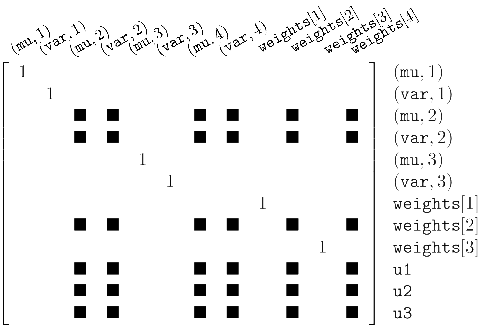
\includegraphics[width=\linewidth]{figures/sparse-jacobian.pdf}
In this case, the Jacobian determinant can be simplified to the determinant of a $6$-by-$6$ matrix that does not grow in size with the number of clusters and number of data points, because unaffected clusters and data points have their values \emph{copied} from the input model trace to the output model trace.
While a reasonable hand-coded implementation of this algorithm would likely exploit this sparsity as well, it would require careful and error-prone reasoning and implementation, which our approach automates.

% TODO show an performance table of moves per second with and without the sparsity reduction (?)

\section{A DYNAMIC CHECK FOR DETECTING BUGS}

Due to the automation described in the previous section, users of Gen can implement involutive MCMC algorithms by writing probabilistic programs for $p$ and $q$ and a differentiable program for the involution $f$, avoiding the need to derive and implement the accept/reject formula by hand. 
This eliminates certain classes of errors that could otherwise be difficult to root out in hand-coded implementations of MCMC algorithms. However, it is still of course possible to implement $p$, $q$, or $f$ incorrectly, introducing bugs that may invalidate the correctness proofs for the involutive MCMC algorithm.


Fortunately, the factorization of diverse algorithms into a common template, involving an explicitly represented model, auxiliary distribution, and involution, enables simple and automated debugging checks that can catch a wide variety of such errors dynamically. These checks are not complete, but anecdotally, we have found that they often alert users to subtle bugs in the design or implementation of an algorithm. The checks are summarized in Algorithm~\ref{alg:dynamic-check}.


\begin{algorithm}[h]
\begin{algorithmic}
\Procedure{imcmc-dynamic-check}{$p$, $q$, $f$}
    \State $x \sim p(\cdot)$ \Comment{Sample state from prior}
    \State $y \sim q_x(\cdot)$ \Comment{Sample auxiliary variables}
    \State $(x', y') \gets f(x, y)$ \Comment{Apply involution}
    \State {\bf assert} $p(x')q_{x'}(y') > 0$ \Comment{Support check}
    \State {\bf assert} $f(x', y') = (x, y)$ \Comment{Involution check}
    \State {\bf assert} $|\text{Rd}^{\textit{cont}}_{f,x,y}| = |\text{Wr}^{\textit{cont}}_{f,x,y}|$ \Comment{Dimension check}
\EndProcedure
\end{algorithmic}
\caption{Dynamic Check for Bugs}
\label{alg:dynamic-check}
\end{algorithm}

To test the user's algorithm, Gen first samples a model trace $x$ from the model prior $p$, and auxiliary randomness $y$ from the kernel $q_x$. It then runs three tests:

\begin{enumerate}
\item \textbf{Support check.} The \textit{support check} runs the involution $f$ on $(x, y)$ and checks that the resulting pair of traces, $(x', y')$, are within the set $Z$ of positive-density elements for $\pi$.

\item \textbf{Involution check.} The \textit{involution check} runs $f \circ f$ on $(x, y)$ and checks that the result is equal to $(x, y)$. If $f$ is an involution on $Z$, then this check will always succeed; if there is a set $\tilde{Z}$ of positive $\pi$-measure on which $f(f(z)) \neq z$ (i.e., $f$ is not an involution), then this check has positive probability of failing.

\item \textbf{Dimension check.} The \textit{dimension check} runs the involution $f$ on $(x, y)$ and records the sets of addresses $\text{Rd}_{f,x,y}^{\textit{cont}}$ and $\text{Wr}_{f,x,y}^{\textit{cont}}$ at which $f$ performs continuous reads and writes, respectively. It then checks that the sizes of these sets match. (Addresses with an $n$-dimensional Lebesgue measure as their reference measure, corresponding to vector-valued random choices, are unpacked into $n$ separate addresses for the purposes of this check.)
\end{enumerate}

These checks each catch qualitatively different bugs in user programs. We now give several examples.

\textit{Incorrectly transformed continuous variables.} Many bugs in the design or implementation of deterministic transformations of continuous variables are naturally detected by the involution check. Consider, for example, the Hamiltonian Monte Carlo algorithm~\citep{hmc}, which, as \citet{imcmc} observe, is an instance of the involutive MCMC framework. 
%$x$ is the model state, $y$ is the momentum, and the involution $f$ first runs a leapfrog integrator to obtain a new state $x'$ and final momentum $-y'$, then negates the final momentum and returns $(x', y')$. 
When applied to HMC, Gen's dynamic bug check involves:
%Gen's dynamic checks will uncover mathematical errors in the implementation of the leapfrog integrator, and will also detect a failure to perform the final negation of the momentum. In particular, the dynamic check involves 
(a) sampling a model state $x$ from the prior; (b) sampling a momentum $y$; (c) running the leapfrog integrator forward to get a new state $x'$ and new momentum $-y'$, (d) running the leapfrog integrator backward from state $x'$ with momentum $y'$, and (e) checking that this results in the state-momentum pair $x, -y$. If the momentum is not properly negated, or if the leapfrog integrator is incorrectly implemented, this check can fail.

As another, simpler example of this type of error, consider the \texttt{split\_params} and \texttt{merge\_params} functions invoked in Figure~\ref{fig:mixture}, as part of a reversible-jump MCMC kernel for learning a mixture of Gaussians with an unknown number of components. Considering only the $\mu$ parameter, suppose the \textit{split} move samples an auxiliary variable $u_1$ and computes $\mu_1 = \mu + u_1, \mu_2 = \mu - u_1$ as the means of the two new clusters. If the \textit{merge} move joins two clusters and assigns $\mu = \sqrt{\mu_1 \mu_2}$, there is a mismatch: a split move cannot be reversed by a corresponding merge, because in general, $\sqrt{(\mu+u_1)(\mu-u_1)} \neq \mu$. This error could be fixed either by changing the split to compute $\mu_1 = \mu u_1, \mu_2 = \frac{\mu}{u_1}$, or by changing the merge to compute $\mu = \frac{\mu_1 + \mu_2}{2}$.

As a final, rather different example in this class, suppose approximate inverses $F_\theta, G_\theta : \mathbb{R}^d \rightarrow \mathbb{R}^d$ are learned neural networks trained via a Cycle GAN objective~\citep{cyclegan} to translate between the latent spaces of two models in a Bayesian model selection problem. A user might implement the following involution:

\begin{center}
\begin{tabular}{c}
{\begin{lstlisting}[basicstyle=\small\ttfamily]
@tracefn h from (tr1, tr2) to (tr3, tr4)
   which_model = @read(tr1, :model, :discrete)
   if which_model == 1
      z = @read(tr1, :z, :continuous)
      z_in_model_2 = F(z)
      @write(tr3, :z, z_in_model_2, :continuous)
      @write(tr3, :model, 2, :discrete)
   else
      z = @read(tr1, :z, :continuous)
      z_in_model_1 = G(z)
      @write(tr3, :z, z_in_model_1, :continuous)
      @write(tr3, :model, 1, :discrete)
   end
end
\end{lstlisting}}
\end{tabular}
\end{center}

However, even though $F_\theta$ and $G_\theta$ are trained with
an objective that encourages $F_\theta(G_\theta(z)) \approx z$, 
this relationship is not exact equality, so the involutive MCMC
framework cannot be directly applied, and the involution check
will fail. This error could be fixed by sampling a proposed value
\textit{near} $F_\theta(z)$ or $G_\theta(z)$, rather than directly applying $F_\theta$
and $G_\theta$ to $z$.

\textit{Discrete logic errors.} Another common class of errors is 
for the discrete logic of an involution to be flawed. Consider the following incorrect 
implementation of a \textit{birth-death} move for the mixture model in Figure~\ref{fig:mixture}, which either adds a new mixture component or selects an existing one
at random to delete:

\begin{center}
\begin{tabular}{c}
{\begin{lstlisting}[basicstyle=\small\ttfamily]
@gen function q(trace)
  current_k = trace[:k]
  is_birth ~ bernoulli(current_k == 1 ? 1.0 : 0.5)
  if is_birth
    new_mu ~ normal(0, 10)
    new_var ~ inv_gamma(1, 10)
  else
    deletion_idx ~ uniform_discrete(1, current_k)
  end
end

@tracefn h from (tr1, tr2) to (tr3, tr4)
   is_birth = @read(tr2, :is_birth, :discrete)
   @write(tr4, :is_birth, !is_birth, :discrete)
   k = @read(tr1, :k, :discrete)
   weights = @read(tr1, :weights, :continuous)
   if is_birth
     @write(tr3, :k, k+1, :discrete)
     new_mu = @read(tr2, :new_mu, :continuous)
     new_var = @read(tr2, :new_var, :continuous)
     @write(tr3, (:mu, k+1), new_mu, :continuous)
     @write(tr3, (:var, k+1), new_var, :continuous)
     new_weights = add_weight(weights)
     @write(tr4, :deletion_idx, k+1, :discrete)
   else
     idx = @read(tr2, :deletion_idx, :discrete)
     @copy(tr1, (:mu, idx), tr4, :new_mu)
     @copy(tr1, (:var, idx), tr4, :new_var)
     for i in (idx+1):k
       @copy(tr1, (:mu, i), tr3, (:mu, i-1))
       @copy(tr1, (:var, i), tr3, (:var, i-1))
     end
     @write(tr3, :k, k-1, :discrete)
     new_weights = delete_weight(weights, idx)
   end
   @write(tr3, :weights, new_weights, :continuous)
end
\end{lstlisting}}
\end{tabular}
\end{center}

The flaw in this implementation is that although the death move can 
delete any of the $k$ mixture components, the birth move can only add
a new component to the \textit{end} (index $k+1$), so the move is not
reversible. Gen's involution check will discover that the deletion of a
component with index $i < k$ is not reversed by a corresponding birth move,
and will thus raise an error.

\textit{Other miscellaneous errors.} When implementing distributions as probabilistic programs, it is also possible for users to make more mundane errors, such as spelling the name of a random choice inconsistently, or characterizing random choices using the wrong \texttt{type} tags (\texttt{:continuous} and \texttt{:discrete}). Such errors can be difficult to detect statically, because the addresses at which a probabilistic program makes random choices, and the distributions of those choices, may change from sample to sample. (Previous work has explored static analyses based on types~\citep{popltraces} and abstract interpretation~\citep{verified_svi}, but these each work on limited subsets of the programs that Gen's full modeling language permits, and it is often precisely these more complex programs that require the flexibility of the involutive MCMC framework in the first place.) Gen's dynamic support and dimension checks can help to detect bugs like these. For example, if the involution $f$ writes to a misspelled address, the support check will determine that the resulting trace's density is 0.

% TODO show an example of the type of bug it can detect (an edge case?)

\textbf{Dynamic checks during inference.} These dynamic assertions can also be run during inference, at each application of the transition kernel. This can be useful to catch bugs that only occur in regions of the state space with low prior mass (but perhaps high posterior mass). When enabled, we can run dynamic checks after each application of the kernel, and when they fail, write to a debugging log and reject the proposed new state. As it turns out, the kernel induced by this procedure is still stationary for $p$:

\begin{lemma}
Let $p$ and $q_x$ be model and auxiliary densities as above, but suppose $f : \mathcal{D} \times \mathcal{D} \rightarrow \mathcal{D} \times \mathcal{D}$ may not be an involution on $Z$.  Trace-based involutive MCMC with dynamic checks enabled, rejecting whenever such a check fails, still yields a kernel that is stationary for $p$.
\end{lemma}
\begin{proof}
Let $R = \{x \in Z \mid f(f(x)) = x \wedge \pi(f(x)) > 0\}$, and let $h(x) := \mathbf{1}[x \in R]f(x) + \mathbf{1}[x \not\in R]x$. Then $h$ is an involution on $Z$, and trace-based involutive MCMC with $p$, $q_x$, and $h$ yields a stationary kernel. But this kernel is the same one induced by using $f$ with dynamic checks. For $x$ on which dynamic checks succeed, $h$ is equivalent to $f$. For $x$ on which dynamic checks fail, $h$ is equivalent to the identity; thus, accepting a move produced by $h$ is equivalent to rejecting.  
\end{proof}

\section{EXAMPLES}

\subsection{Reversible Jump MCMC}
Reversible jump MCMC~\citep{green1995reversible,hastie2012model} is a special case of involutive MCMC, and 
the implementation of reversible jump MCMC kernels can be automated using the probabilistic and differentiable programming languages presented in this paper.
We now review reversible jump MCMC, then show how it can be automated using the techniques presented earlier, and give an example.

The reversible jump MCMC framework involves a set of `models' $k \in \mathcal{K}$, and a prior distribution on models $p(k)$.
For each model, there is a latent continuous parameter vector $\theta_k \in \mathbb{R}^{n(k)}$ where $n(k)$ is the dimension of model $k$, and a likelihood function $L_{D,k}(\theta_k)$ for each $k$ given data $D$.
The latent state $x$ is a pair $(k, \theta_k)$ of model and continuous parameter.
There is a set of \emph{move types} $\mathcal{M}$.
Each move type $m \in \mathcal{M}$ is associated with an unordered pair of models $(k_1, k_2)$ and a dimensionality $d(m)$ such that $d(m) \ge n(k_1)$ and $d(m) \ge n(k_2)$ (zero, one, or more than one move types maybe assocaite with a given pair of models).
For each latent state $x = (k, \theta_k)$, there is a probability distribution $q_{x}(m)$ on move types such that $q_{x}(m) > 0$ implies that $k$ is one of the models for move type $m$.
For each move type $m \in \mathcal{K}$ between $k_1$ and $k_2$ there is a pair of continuously differentiable bijections $h_{m, k_1 \to k_2} : \mathbb{R}^{d(m)} \to \mathbb{R}^{d(m)}$ and $h_{m, k_2 \to k_1} := h_{m, k_1 \to k_2}^{-1}$, and a pair of proposal densities $q_{m,k_1 \to k_2}(u_{k_1 \to k_2})$ and $q_{m,k_2 \to k_1}(u_{k_2 \to k_1})$ where $u_{k_1 \to k_2} \in \mathbb{R}^{d(m) - n(k_1)}$ and $u_{k_2 \to k_1} \in \mathbb{R}^{d(m) - n(k_2)}$.
A proposal is made from state $x = (k, \theta_k)$ by (i) sampling a move type $m \sim q_{x}(\cdot)$, and (ii) sampling continuous variable $u \sim q_{m,k \to k'}(\cdot)$ for $(k, k')$ associated with $m$, and (iii) computing $(\theta_{k}', u') := h_{m,k \to k'}(\theta_k, u)$, and proposing new state $x' = (k', \theta_k')$.
The move is accepted with probability:
\begin{equation}
{
\min\left\{ 1,
\frac{p(k')}{p(k)} \frac{p_{k'}(\theta_{k'})}{p_k(\theta_k)} \frac{L_{D,k'}(\theta_k')}{L_{D,k}(\theta_k)}
\frac{q_{x'}(m)}{q_{x}(m)}
\frac{q_{m,k' \to k}(u)}{q_{m,k \to k'}(u)}
\right\}
}
\end{equation}

To represent reversible jump MCMC using involutive MCMC implemented with probabilistic programs, we write a probabilistic program $P$ that encodes the space of models $\mathcal{K}$, the prior distribution on models, $p(k)$, the per-model priors $p_k(\theta_k)$ and the per-model likelihoods $L_{D,k}(\theta_k)$.
The set of all models $k$ corresponds to the set of all pairs $(A_P, \mathbf{d}_P)$ where $A_P$ represent possible trace structures (i.e. control-flow paths through $P$) and $\mathbf{d}_P$ are the set of assignments to discrete random choices made by $P$.
The per-model continuous parameters $\theta$ correspond to continuous random choices $\mathbf{c}_P$.
% TODO explain the likelihood
An auxiliary probabilistic program $Q$ encodes both the probability distribution on moves types using discrete random choices and possibly stochastic control flow ($(A_Q, \mathbf{d}_Q)$), and the per-move-type probability densities on $u$ using continuous random choices $\mathbf{c}_Q$.
The involution $f$ factors into an (i) involution $f_1$ on pairs $i = ((A_P, \mathbf{d}_P), (A_Q, \mathbf{d}_Q))$ that defines the association between move types $\mathcal{M}$ and the model pairs ($k_1, k_2$); and (ii) a family of bijections $f_{1,i}$ on the space of pairs $(\mathbf{c}_P, \mathbf{c}_Q)$ of continuous random choices for both programs for fixed values of the discrete random choices and fixed trace structure.

Figure~\ref{fig:mixture} shows a split-merge reversible jump kernel for an infinite Gaussian mixture model~\citep{richardson1997bayesian} implemented using the probabilistic and differentiable programming languages described in this paper.
Figure~\ref{fig:mixture}(b) shows the infinite Gaussian mixture model, specified as a probabilistic program $P$.
The program takes the number of data points as input, then samples the number of clusters from a Poisson distribution, then samples cluster parameters and mixture proportions, and finally samples the data points from the resulting finite mixture.
Figure~\ref{fig:mixture}(c) shows the auxiliary probabilistic program $Q$ for the split-merge kernel.
This program takes a trace of the model program as input, and randomly decides whether to split a cluster and increase the number of clusters by one or merge two clusters and decrease the number of clusters by one.
Then, the program randomly picks which cluster to split, or which clusters to merge.
This kernel always merges the last cluster with a random other cluster; for ergodicity the move can be composed with a simple move (that has acceptance probability $1$) that swaps a random cluster with the last cluster.
If a split is chosen, then the program also samples the three degrees of freedom necessary to generate the new parameters for the clusters in an invertible manner.
Figure~\ref{fig:mixture}(d) shows a differentiable program specifying the involution for the split-merge kernel, and Figure~\ref{fig:mixture}(f) shows graphically how this involution acts on pairs of traces.
The yellow section (1) defines an involution $f_1$ on the discrete random choices that specifies that (i) the \texttt{split} choice should be flipped (so that split moves are always mapped to merge moves and vice versa) and that (ii) the number of clusters should be increased by one for a split move and decreased by one for a merge move, and (iii) which merged cluster corresponds to which split clusters.
The green section (2) specifies the continuous bijections that govern the transformation of continuous random choices during split moves and the purple section (3) specifies the inverses of these bijections, which govern the transformation of continuous choices during merge moves.

\subsection{State-Dependent Mixture Proposal}

State-dependent mixture proposal.
Depending on the current state of the model, a different mixture distribution is used for the proposal.
Implementing such a move requires computing the mixture probability under the forward move and under the reverse move, which may differ.

$q_x(m)$ -- the mixture distribution

$q_m(x')$ -- the proposal we are mixing over

The first part of the auxiliary probabilistic program $Q$ determines which proposal to apply by sampling from a mixture distribution.
Here, the program picks a random node in the tree, by doing a stochastic walk of the tree that terminates at the chosen node.
\begin{center}
\begin{tabular}{c}
{\begin{lstlisting}[basicstyle=\small\ttfamily]
prev_cov_function = trace[:cov_function]
path ~ walk_tree(prev_cov_function, ..)
\end{lstlisting}}
\end{tabular}
\end{center}
The first part of the involution copies the random choices corresponding to the mixture from the input auxiliary trace to the output auxiliary trace.
\begin{center}
\begin{tabular}{c}
{\begin{lstlisting}[basicstyle=\small\ttfamily]
@copy(q_in, :path, q_out, :path)
\end{lstlisting}}
\end{tabular}
\end{center}

The code that walks the tree uses the following recursion, which results in a probability distribution that assigns exponentially lower probability to nodes that are deeper in the tree.
\begin{center}
\begin{tabular}{c}
{\begin{lstlisting}[basicstyle=\small\ttfamily]
if ({:done} ~ bernoulli(0.5))
  return path
elseif ({:recurse_left} ~ bernoulli(0.5))
  path = (path..., :left_node)
  return ({:left} ~ walk_tree(node.left, path))
else
  path = (path..., :right_node)
  return ({:right} ~ walk_tree(node.right, path))
end
\end{lstlisting}}
\end{tabular}
\end{center}
The resulting mixture distributions for two trees are:
\begin{center}
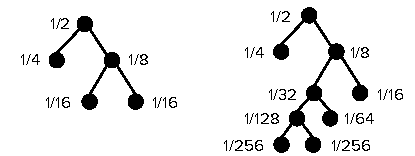
\includegraphics[width=0.8\linewidth]{figures/biased-tree-distribution.pdf} % TODO improve quality
\end{center}
Because the mixture is specified using a probabilistic program, it is straightforward to modify the program to define a different mixture distribution.
The code below specifies a mixture distribution that is uniform over all nodes in the tree.
\begin{center}
\begin{tabular}{c}
{\begin{lstlisting}[basicstyle=\small\ttfamily]
n1 = size(node.left); n2 = size(node.right)
if ({:done} ~ bernoulli(1 / (1 + n1 + n2)))
  return path
elseif ({:recurse_left} ~ bernoulli(n1 / (n1+n2))
  path = (path..., :left_node)
  return ({:left} ~ walk_tree(node.left, path))
else
  path = (path..., :right_node)
  return ({:right} ~ walk_tree(node.right, path))
end
\end{lstlisting}}
\end{tabular}
\end{center}
The resulting distributions are:
\begin{center}
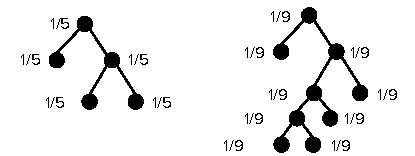
\includegraphics[width=0.8\linewidth]{figures/unbiased-tree-distribution.pdf}
\end{center}
Note that in the first case, the ratio of mixture probabilities is either $1$, $0.5$, or $2$ depending on whether the previous and new subtrees are leaf or internal nodes.
In the second case, the ratio of mixture probabilities is the ratio of sizes of the two trees.
%Automating the computation of the mixture probabilities




The rest of the kernel specifies what happens for each chosen node.
The second part of the auxiliary probabilistic program $Q$ implements a common motif for Metropolis-Hastings algorithms, where the proposal samples new values for some random choices:
\begin{center}
\begin{tabular}{c}
{\begin{lstlisting}[basicstyle=\small\ttfamily]
new_subtree ~ cov_function_prior()
\end{lstlisting}}
\end{tabular}
\end{center}
and the involution swaps the old value with the newly proposed value:
\begin{center}
\begin{tabular}{c}
{\begin{lstlisting}[basicstyle=\small\ttfamily]
@copy(p_in, subtree_address, q_out, :new_subtree)
@copy(q_in, :new_subtree, p_out, subtree_address)
\end{lstlisting}}
\end{tabular}
\end{center}
Here the values happen to be trees that themselves have a random number of random choices, but the same motif is also used in simpler applications of Metropolis-Hastings.


Here, the proposal we are mixing over is easy to implement -- it involvs resampling a subtree from the prior, so the Jacobian is 1 and there is cancellation between the model and the proposal.

But computing the mixture probabilities is complex, because the mixture is a mixture of either $n_1$ or $n_2$ elements, which depends on the size of the tree.

Show the mixture probabilities in math notation?
If both subtrees not leaf nodes, then the probabilities are the same.
If both subtrees are leaf nodes, then the probabilities are different.
If one subtree is a leaf node and the other is an internal node then the ratio is either $0.5$ or $2$ respectively.
\begin{equation}
q
\end{equation}

TODO: relate to `resimulation Metropolis-Hastings' in general-purpose probabilistic programs.

Of course, it is straightforward to replace the prior with a custom data-driven proposal distribution on subtrees.

\subsubsection*{Acknowledgements}
All acknowledgments go at the end of the paper, including thanks to reviewers who gave useful comments, to colleagues who contributed to the ideas, and to funding agencies and corporate sponsors that provided financial support.

\bibliography{references} 

\clearpage
\onecolumn
\section*{APPENDIX}

%\subsection{Distributions on traces}
%% TODO rewrite this section..
%Define target density $\pi$ (XXX below it is called $p$, fix this) on the joint space $X \times U$, where $X$ are traces of the model and $X$ are traces of the proposal, in terms of the density $p(x)$ and the family of densities $q_x(u)$ as $\pi(x, u) := p(x) q_u(x)$.
%
%% TODO rename the joint target density to \pi below
%We want to show stationarity with respect to $\pi$, using stationarity of the involution with respect to the joint density (below).
%\begin{equation}
%\int_X p(x) \ell_x(A) \mu(dx) = p(A) \mbox{ for all } A \in \Sigma
%\end{equation}
%where $\ell_x(A)$ is the probability of transitioning into set $A$ from $x$, and is given by:
%\begin{equation}
%\ell_x(A) := \int_U k_{(x, u)}(A \times U) \mu(du)
%\end{equation}
%where $k_{(x, u)}$ is the measure on $X \times U$ that is induced by applying the involution $h$ to the state $(x, u)$.
% TODO checkme


\subsection{Derivation of the pushforward Radon-Nikodym derivative for a special case} \label{sec:radon-nikodym-special-case}
Implementing Algorithm~\ref{alg:involutive-mcmc} requires computing the Radon-Nikodym derivative $d (\mu \circ f^{-1}) / d \mu$.
This section derives that function for the special case in which the involution $f$ can be factored into an involution on a countable set $I$ and a family of bijections on $\mathbb{R}^{n_i}$ for some $n_i$ for each $i \in I$.
Suppose $Z = \{(i, \mathbf{x}) : i \in I, \mathbf{x} \in \mathbb{R}^{n_i}\}$.
Suppose $f_1$ is an involution on $I$ and $n_i = n_{f_1(i)}$ and $f_2$ is a family of continuously differentiable bijections indexed by $i \in I$, such that $f_{2,i} : \mathbb{R}^{n_i} \to \mathbb{R}^{n_i}$.
Also suppose that $f_{2,i} = f_{2,f_1(i)}^{-1}$ for all $i \in I$. That is,
\begin{equation}
f_{2,i}(f_{2,f_1(i)}(\mathbf{x})) = \mathbf{x} \mbox{ for all } \mathbf{x} \in \mathbb{R}^{n_i} \mbox{ and all } i \in I
\end{equation} 
Then, $f : Z \to Z : (i, \mathbf{x}) \mapsto (f_1(i), f_{2,i}(\mathbf{x}))$ is an involution because:
\begin{equation}
f(f(i, \mathbf{x})) = f(f_1(i), f_{2,i}(\mathbf{x})) = (f_1(f_1(i)), f_{2,f_1(i)}(f_{2,i}(\mathbf{x}))) = (i, \mathbf{x})
\end{equation}
Let $\Sigma_n$ and $\mu_n$ denote the Lebesgue $\sigma$-algebra and Lebesgue measure on $\mathbb{R}^n$, respectively.
Let $\Sigma \subset \mathcal{P}(Z)$ be the $\sigma$-algebra of sets of the form $\cup_{i \in I} \{(i, \mathbf{x}) : \mathbf{x} \in A_i\}$ for some $A_i \in \Sigma_{n_i}$ for each $i \in I$.
%Let $\Sigma$ be the $\sigma$-algebra on $Z$ generated by the sets $G := \{ \{(i, \mathbf{x}) : \mathbf{x} \in A\} : i \in I, A \in \Sigma_{n_i} \}$.
%Note that the sets $G$ form a $\pi$-system:
%\begin{align}
%\{(i, \mathbf{x}) : \mathbf{x} \in A\} \cap \{(j, \mathbf{x}) : \mathbf{x} \in B\} = \varnothing = \{(i, \mathbf{x}) : \mathbf{x} \in \varnothing \} \in G \mbox{ for } i \ne j\\
%\{(i, \mathbf{x}) : \mathbf{x} \in A\} \cap \{(i, \mathbf{x}) : \mathbf{x} \in B\} = \{(i, \mathbf{x}) : \mathbf{x} \in A \cap B\} \in G \mbox{ because } A \cap B \in \Sigma_{n_i}
%\end{align}
Let $\mu$ denote the measure on measurable space $(Z, \Sigma)$ given by:%, uniquely defined by its value on the sets $G$:
\begin{equation}
\mu(\cup_{i \in I} \{(i, \mathbf{x}) : \mathbf{x} \in A_i\}) := \sum_{i \in I} \mu_{n_i}(A_i)
\end{equation}
We wish to show that the Radon-Nikodym derivative of the pushforward of $\mu$ by $f$ with respect to $\mu$, evaluated at $(i, \mathbf{x})$, is the absolute value of the Jacobian (determinant) of the function $f_{2,i}$ evaluated at $\mathbf{x}$, which is denoted $(J f_{2,i})(\mathbf{x})$:
\begin{equation}
\frac{d (\mu \circ f^{-1})}{d \mu}(i, \mathbf{x})
= \left| (Jf_{2,i})(\mathbf{x})\right|
\end{equation}
Consider $(\mu \circ f^{-1})(A)$ for $A \in \Sigma$:
\begin{align}
(\mu \circ f^{-1})(\cup_{i \in I} \{ (i, \mathbf{x}) : \mathbf{x} \in A_i \})
&= \mu(f^{-1}(\cup_{i \in I} \{ (i, \mathbf{x}) : \mathbf{x} \in A_i \}))\\
&= \mu(\cup_{i \in I} f^{-1}(\{ (i, \mathbf{x}) : \mathbf{x} \in A_i \}))\\
&= \mu(\cup_{i \in I} \{ (f_1(i), \mathbf{x}) : \mathbf{x} \in f_{2,i}(A_i) \})\\
&= \sum_{i \in I} \mu_{n_i}(f_{2,i}(A_i))
\end{align}
It suffices to show that for all $A \in \Sigma$:
\begin{equation}
\int_A \left| (Jf_{2,i})(\mathbf{x})\right| \mu(dz) = \sum_{i \in I} \mu_{n_i}(f_{2,i}(A_i))
\end{equation}
Expanding the left-hand side:
\begin{align}
\int_A \left| (Jf_{2,i})(\mathbf{x})\right| \mu(dz)
= \sum_{i \in I} \int_{A_i} \left| (Jf_{2,i})(\mathbf{x})\right| \mu_{n_i}(d \mathbf{x}) % TODO how to justify this? it seems obvious
= \sum_{i \in I} \mu_{n_i}(f_{2,i}(A_i)) % Borgachev Theorem 4.7.1 
\end{align}
where the final step uses Borgachev Theorem 3.7.1 with $g := 1$, and $F := f_{2,i}$.

\subsection{Proof of detailed balance for involution} \label{sec:involution-detailed-balance}

\begin{lemma}
Given $\sigma$-finite measures $(X_P, \Sigma_P, \mu_P)$ and $(X_Q, \Sigma_Q, \mu_Q)$,
if $X \in \Sigma_P \otimes \Sigma_Q$ then $\Sigma = \{A \in \Sigma_P \otimes \Sigma_Q : A \subseteq X\}$ is a $\sigma$-algebra on $X$, and $\mu : \Sigma \to [0, \infty)$ given by $\mu(A) := (\mu_P \times \mu_Q)(A)$ is $\sigma$-finite measure on measurable space $(X, \Sigma)$.
\end{lemma}
\begin{proof}
TODO: write out the detailed steps, proving each property of a $\sigma$-algebra%$ TODO
\end{proof}

\begin{lemma}
$\pi : X \to [0, \infty)$ is a probability density with respect to $\mu$ and the measure induced by $\pi$ and the measure $\mu$ are mutually absolutely continuous 
\end{lemma}
\begin{proof}
% TODO need to show that pi is measurable by the product measure?
\begin{equation}
\int_X \pi(x) \mu(dx) = \int_{X_P \times X_Q} \pi(x) (\mu_P \times \mu_Q)(dx) = \int_{X_P} p(t) \left( \int_{X_Q} q_t(u) \mu_Q(du) \right) \mu_P(dt) = 1
\end{equation}

%(note that $\mu$ is $\sigma$-finite since $\mu_P \times \mu_Q$ is $\sigma$-finite. % TODO: prove this 
%Suppose that $\pi$ is a probability density with respect to $\mu$. % TODO is this guaranteed?
\end{proof}


\citet{tierney1998note} gives a class of MCMC kernels based on involutions that satisfy detailed balance.
We reproduce the result in our notation:
\begin{lemma}[Detailed balance for involution move~\citep{tierney1998note}] \label{lemma:tierney-involution}
Let $(Z, \Sigma, \pi)$ denote a measure space.
Suppose $f$ is a one-to-one function from $Z$ onto $Z$ such that $f^{-1} = f$.
Consider the probability kernel $k$ defined by $k_z(A) := [f(z) \in A] \alpha(z, f(z)) + [z \in A] (1 - \alpha(z, f(z)))$ (where $\alpha(z, f(z))$ gives the probability of accepting a proposed transition from $z$ to $f(z)$).
Let $\nu(dz) := \pi(dz) + (\pi \circ f^{-1})(dz)$.
Let $h(z)$ be a density for $\pi$ with respect to $\nu$.
Let $A := \{z \in Z : h(z) > 0 \mbox{ and } h(f(z)) > 0\}$.
$k$ satisfies detailed balance with respect to $\pi$ if and only if:
\begin{enumerate}
\item $\alpha(z, f(z)) = 0$ for $\pi$-almost all $z \not \in A$
\item $\alpha(z, f(z)) \frac{h(z)}{h(f(z))} = \alpha(f(z), z)$
\end{enumerate}
\end{lemma}

Now we apply Lemma~\ref{lemma:tierney-involution} to our setting where $\pi$ is $\sigma$-finite, there exists a $\sigma$-finite reference measure $\mu$ for measurable space $(Z, \Sigma)$ such that $\pi$ is mutually absolutely continuous with respect to $\mu$, and where the pushforward of $\mu$ by $f$, denoted $\mu \circ f^{-1}$, is absolutely continuous with respect to $\mu$.
%(One step in the proof---Equation~\ref{eq:mu-is-absolutely-continuous-with-respect-to-nu}---will also require that $\mu$ is also absolutely continuous with respect to $\pi$, which is possible if we restrict $Z$ to the support of $\pi$, $\{z : (d \pi / d \mu)(z) > 0\}$, which must be in the $\sigma$-algebra $\Sigma$).

In our setting, $\alpha$ is defined as:
\begin{equation}
\alpha(z, f(z)) := \mbox{min}\left\{1, \frac{\frac{d \pi}{d \mu}(f(z))}{\frac{d \pi}{d \mu}(z)} \cdot \frac{d (\mu \circ f^{-1})}{d \mu}(z)\right\}
\end{equation}
This definition of $\alpha$ satisfies:
\begin{equation}
\alpha(z, f(z)) \frac{\frac{d \pi}{d \mu}(z)}{\frac{d \pi}{d \mu}(f(z))} \cdot \left( \frac{d (\mu \circ f^{-1})}{d \mu} (z)\right)^{-1}= \alpha(f(z), z)
%\frac{\alpha(z, f(z))}{\alpha(f(z), z)} = \frac{\pi(T(z))}{\pi(z)} \left( \frac{d (\mu \circ T^{-1})}{d \mu} (z) \right)
\end{equation}
Therefore, to apply Lemma~\ref{lemma:tierney-involution}, it suffices to show $\pi$ has density with respect to $\nu$ (denoted $h(z)$) such that:
\begin{equation}
\frac{h(z)}{h(f(z))} = \frac{\frac{d \pi}{d \mu}(z)}{\frac{d \pi}{d \mu}(f(z))} \left( \frac{d (\mu \circ f^{-1})}{d \mu} (z)\right)^{-1}
\end{equation}
Since $\pi$ and $\pi \circ f^{-1}$ are both absolutely continuous with respect to $\mu$, $\nu$ is also absolutely continuous with respect to $\mu$, and has density:
\begin{equation}
\frac{d \nu}{d \mu}(z) = \frac{d \pi}{d \mu}(z) + \frac{d (\pi \circ f^{-1})}{d \mu}(z) 
\end{equation}
$\pi$ is absolutely continuous with respect to $\nu$, and therefore:
\begin{equation}
\frac{d \pi}{d \mu}(z) = \frac{d \pi}{d \nu}(z) \cdot \frac{d \nu}{d \mu}(z)
\end{equation}
Because $(d \pi / d \mu)(z) > 0$ for all $z \in Z$, $(d \nu / d \mu)(z) > 0$ for all $z \in Z$.
Therefore,
\begin{equation}
h(z)
:= \frac{d \pi}{d \nu}(z)
= \frac{\frac{d \pi}{d \mu}(z)}{\frac{d \nu}{d \mu}(z)}
\end{equation}
Therefore:
\begin{equation}
\frac{h(z)}{h(f(z))} = \frac{\frac{d \pi}{d \mu}(z)}{\frac{d \pi}{d \mu}(f(z))} \cdot \frac{\frac{d \nu}{d \mu}(f(z))}{\frac{d \nu}{d \mu}(z)}
\end{equation}
It suffices to show that:
\[
\frac{\frac{d \nu}{d \mu}(f(z))}{\frac{d \nu}{d \mu}(z)} = \left(\frac{d (\mu \circ f^{-1})}{d \mu}(z)\right)^{-1}
\]

First, we prove a Lemma:
\begin{lemma} \label{lemma:reference-measure-pushforward}
If $(Z, \Sigma)$ is a measurable space and $f : Z \to Z$ is a measurable function that is an involution, $\nu$ and $\mu$ are $\sigma$-finite measures such that $\nu$ is absolutely continuous with respect to $\mu$, and such that the pushforward measures $\nu \circ f^{-1}$ and $\mu \circ f^{-1}$ are both $\sigma$-finite, then
$\nu \circ f^{-1}$ is absolutely continuous with respect to $\mu \circ f^{-1}$ and
\begin{equation}
\frac{d (\nu \circ f^{-1})}{d (\mu \circ f^{-1})}(z) = \frac{d \nu}{d \mu}(f(z))
\end{equation}
\end{lemma}
\begin{proof}
First, $\nu \circ f^{-1}$ is absolutely continuous with respect to $\mu \circ f^{-1}$ because
$(\mu \circ f^{-1})(A) = 0$ implies $\mu(f^{-1}(A)) = 0$ implies $\nu(f^{-1}(A)) = 0$ implies $(\nu \circ f^{-1})(A) = 0$.
To show that $z \mapsto (d \nu / d \mu)(f(z))$ is the Radon-Nikodym derivative $d (\nu \circ f^{-1}) / d (\mu \circ f^{-1})$, it suffices to show that for all $A \in \Sigma$:
\begin{equation}
\int_A \left( \frac{d \nu}{d \mu} (f(z)) \right) ( \mu \circ f^{-1} )(dz) = (\nu \circ f^{-1})(A) := \nu(f^{-1}(A))
\end{equation}
Applying Theorem 3.6.1 in Bogachev with $Y := A$, $y := z$, $x := z'$, $X := f^{-1}(A)$, and $g(y) := (d\nu / d\mu)(f(y))$:
\begin{align}
\int_A \left( \frac{d \nu}{d \mu} (f(z)) \right) ( \mu \circ f^{-1} )(dz)
&= \int_Y g(y) ( \mu \circ f^{-1} )(dy)\\
&= \int_X g(f(x)) \mu(dx) \;\;\;\; [\mbox{Bogachev Theorem 3.6.1}]\\
&= \int_{f^{-1}(A)} (d\nu / d\mu)(f(f(z'))) \mu(dz')\\
&= \int_{f^{-1}(A)} (d\nu / d\mu)(z') \mu(dz')\\
&= \int_{f^{-1}(A)} \nu(dz')
= \nu(f^{-1}(A))
\end{align}
% NOTE Bogachev's theorem uses domains of integration which are the whole
% sample spaces for the two sigma algebras.  I think that the theorem should
% also apply to any measurable sets A and T(A) because one can construct a
% sigma algebra and measure that are restricted to to any nonempty measurable
% set.

\end{proof}

Now, note that $\nu$ and $\nu \circ f^{-1}$ are the same measure:
\begin{align}
\nu(A) &= \pi(A) + \pi'(A) = \pi(A) + \pi(f^{-1}(A))\\
(\nu \circ f^{-1})(A) &= \pi(f^{-1}(A)) + \pi(f^{-1}(f^{-1}(A))) = \pi(f^{-1}(A)) + \pi(A)
\end{align}
Therefore,
\[
\frac{d (\nu \circ f^{-1})}{d \nu}(z) = 1 \mbox{ for all } z
\]
Expanding $d(\nu \circ f^{-1}) / d \nu$ using the chain rule:
\begin{align}
1 &= \frac{d (\nu \circ f^{-1})}{d \nu}(z)\\
&=   \frac{d (\nu \circ f^{-1})}{d (\mu \circ f^{-1})}(z) \cdot
    \frac{d (\mu \circ f^{-1})}{d \mu}(z) \cdot
    \frac{d \mu}{d \nu}(z) \label{eq:mu-is-absolutely-continuous-with-respect-to-nu}\\
&= \frac{d \nu}{d \mu}(f(z)) \cdot \frac{d (\mu \circ f^{-1})}{d \mu}(z) \cdot \frac{d \mu}{d \mu}(z) \;\;\;\; [\mbox{Lemma~\ref{lemma:reference-measure-pushforward}}]\\
&= \frac{d \nu}{d \mu}(f(z)) \cdot \frac{d (\mu \circ f^{-1})}{d \mu}(z) \cdot \frac{1}{\frac{d \nu}{d \mu}(z)}\\
\left(\frac{d (\mu \circ f^{-1})}{d \mu}(z)\right)^{-1} &= \frac{\frac{d \nu}{d \mu}(f(z))}{\frac{d \nu}{d \mu}(z)}
\end{align}

\subsection{Proof of stationarity for involution} \label{sec:involution-is-stationary}
Detailed balance of the the involution kernel with respect to the measure induced by $\pi$ implies:
\begin{equation}
\int_B \pi(z) k'_z(A) \mu(dz) = \int_A \pi(z) k'_z(B) \mu(dz) \;\; \mbox{ for all } A, B \in \Sigma
\end{equation}
Stationarity with respect to $\pi$ follows by substituting $Z$ for $B$:
\begin{align}
\int_Z \pi(z) k'_z(A) \mu(dz) &= \int_A \pi(z) k'_z(Z) \mu(dz) = \int_A \pi(z) \mu(dz) \;\; \mbox{ for all } A \in \Sigma\\
\end{align}

\subsection{Proof of stationarity for end-to-end kernel} \label{sec:involutive-mcmc-is-stationary}
We are given that the involution is stationary with respect to (the measure induced by) $\pi(x, u) := p(x) q_x(u)$:
\begin{equation}
\int_Z k'_z(A) \pi(z) \mu(dz) = \int_A \pi(z) \mu(dz) \mbox{ for all } A \in \Sigma
\end{equation}
The end-to-end kernel is defined fir all $x \in X_P$ such that $p(x) > 0$ as:
\begin{equation}
k_x(A) := \int_U k'_{x,u}(A \times U) q_x(u) \mu_U(du) \;\; \mbox{for all} \;\; A \in \Sigma_P, x \in X
\end{equation}
Stationarity of the end-to-end kernel with respect to the measure induced by $p$ is:
\begin{equation}
\int_X k_x(A) p(x) \mu_P(dx) = \int_A p(x) \mu_P(dx) \mbox{ for all } A \in \Sigma_P
\end{equation}
Expanding:
\begin{align*}
    \int_X k_x(A) p(x) \mu_P(dx) &= \int_X \left( \int_U k'_{x,u}(A \times U) q_x(u) \mu_Q(du) \right) p(x) \mu_P(dx)\\
    &= \int_{X \times U} k'_{x,u}(A \times U) q_x(u) p(x) (\mu_P \times \mu_Q)(dz) \;\; [\mbox{ Tonelli's theorem }]\\ % TODO check
    &= \int_{Z} k'_{x,u}(\{(x', u') \in Z : x' \in A\}) \pi(z) \mu(dz)\\ % TODO justify
    &= \int_{\{(x, u) \in Z : x \in A\}} \pi(z) \mu(dz)\;\;\; [\mbox{ Stationarity of $k'$ with respect to $\pi$}]\\
    &= \int_{\{(x, u) \in Z : x \in A\}} q_x(u) p(x) \mu(dz)\\
    &= \int_A \left( \int_U q_x(u) \mu_Q(du) \right) p(x) \mu_P(dx)\\
    &= \int_A p(x) \mu_P(dx)
\end{align*}
% TODO characterize the various assumptions that allow us to e.g. rearrange the order of integration, etc.

%\paragraph{Proof of stationarity}
%We need the composition of the two programs to define a valid probabilistic program with density $\pi$ that is absolutely continuous with respect to the refernce measure $\mu$.
%We also need there to be a particular relationship between $\pi$ and $p$.
%The involution part of the kernel is a kernel on the combined space $(Z, \Sigma_Z, \mu)$.
%\[
%k'_z(B_Z) = [f(z) \in B_Z] \alpha(z) + [z \in B_Z] (1 - \alpha(z))
%\]
%The kernel of Algorithm 1 is defined by:
%\[
%k_t(B_T) := \int_{U_t} q_{t}(u) k'_{(t, u)}(\{(t', u') \in Z : t' \in B_T\}) \mu_{Q,t}(du)
%\]
%We want to show it is stationary:
%\begin{align}
%\int_T k_t(B_T) p(t) \mu_P(dt) &= p(B_T) \mbox{ for all } B_T \in \Sigma_P\\
%\int_T \left( \int_{U_t} q_{t}(u) k'_{(t, u)}(\{(t', u') \in Z : t' \in B_T\}) \mu_{Q,t}(du) \right) p(t) \mu_P(dt) &= p(B_T)\\
%\sum_{i} \int_{T_C} \left( \int_{U_t} q_{t}(u) k'_{(t, u)}(\{(t', u') \in Z : t' \in B_T\}) \mu_{Q,t}(du) \right) p(i, t_c) \mu_{P_C,i}(dt_c) &= p(B_T)\\ % separate out discrete part of t (i) and continuous part of t (t_c)
%\sum_{i} \int_{T_C} \left( \int_{U_i} q_{t}(u) k'_{(t, u)}(\{(t', u') \in Z : t' \in B_T\}) \mu_{Q,i}(du) \right) p(i, t_c) \mu_{P_C,i}(dt_c) &= p(B_T)\\ % use that the reference measure mu_{Q,t} only depends on the discrete part
%..\\
%\int_{Z} \pi(t, u) k'_{t,u}(\{(t', u') \in Z : t' \in B_T\}) \mu(dz) &= p(B_T)\\
%\pi(\{(t', u') \in Z : t' \in B_T\}) &= p(B_T)\\
%\end{align}
%
%the set of addresses $\mathcal{A}$ is partitioned into two spaces $\mathcal{A}_1$ and $\mathcal{A}_2$\\
%
%each structure $S$ partitions into two structures $S_1$ and $S_2$
%
%then $Z := \cup_{S \in \mathcal{S}} \{(S, \mathbf{x}) : \mathbf{x} \in \times_{a \in S} X_a \}$\\
%
%Space for $Z$:
%\[
%\cup_{S \in \mathcal{S}} \{((\mathcal{A}_1 \cap S) \cup (\mathcal{A}_2 \cap S), \mathbf{x_1}, \mathbf{x_2}) : \mathbf{x_1} \in \times_{a \in S_1} X_a, \mathbf{x_2} \in \times_{a \in S_2} X_a\}
%\]
%
%Space for $T$:
%\[
%\cup_{S_1 \in \mathcal{S}} \{(S_1, \mathbf{x_1}) : \mathbf{x_1} \in \times_{a \in S_1}\}
%\]
%
%\begin{align}
%\pi(
%\cup_{S \in \mathcal{S} : A_1 \cap S = S_1} \{(S_1 \cup (\mathcal{A}_2 \cap S), \mathbf{x_1}, \mathbf{x_2}) : \mathbf{x_1} \in B_{S_1}, \mathbf{x_2} \in \times_{a \in S_2} X_a\}
%) &= p(B_T)\\
%\sum_{S \in \mathcal{S} : A_1 \cap S = S_1} \int_{B_{S_1} \times \otimes_{a \in S_2} X_a} \pi(S_1, S_2, \mathbf{x}_1, \mathbf{x}_2) \mu_{S_1 \cup S_2}(d \mathbf{x}_1 \mathbf{x}_2) &= p(B_T)\\
%\sum_{S \in \mathcal{S} : A_1 \cap S = S_1} \int_{B_{S_1} \times \otimes_{a \in S_2} X_a} p(S_1, \mathbf{x}_1) q_{(S_1,\mathbf{x}_1)}(S_2, \mathbf{x}_2) \mu_{S_1 \cup S_2}(d \mathbf{x}_1 \mathbf{x}_2) &= p(B_T)\\
%\sum_{S \in \mathcal{S} : A_1 \cap S = S_1} \int_{B_{S_1}} p(S_1, \mathbf{x}_1) \left( \int_{\otimes_{a \in S_2 X_a}} q_{(S_1,\mathbf{x}_1)}(S_2, \mathbf{x}_2) \mu_{S_2}(d \mathbf{x}_2) \right) \mu_{S_1}(d \mathbf{x}_1) &= p(B_T) [\mbox{Fubini / Tonnelli?}]\\
%\sum_{S_2 \subseteq A_2 : S_1 \cup S_2 \in \mathcal{S}} \int_{B_{S_1}} p(S_1, \mathbf{x}_1) \left( \int_{\otimes_{a \in S_2 X_a}} q_{(S_1,\mathbf{x}_1)}(S_2, \mathbf{x}_2) \mu_{S_2}(d \mathbf{x}_2) \right) \mu_{S_1}(d \mathbf{x}_1) &= p(B_T)\\
%\int_{B_{S_1}} p(S_1, \mathbf{x}_1) \left( \sum_{S_2 \subseteq A_2 : S_1 \cup S_2 \in \mathcal{S}} \int_{\otimes_{a \in S_2 X_a}} q_{(S_1,\mathbf{x}_1)}(S_2, \mathbf{x}_2) \mu_{S_2}(d \mathbf{x}_2) \right) \mu_{S_1}(d \mathbf{x}_1) &= p(B_T) [\mbox{Fubini / Tonnelli?}]\\
%\end{align}
%It suffices to show that
%\begin{align}
%\sum_{S_2 \subseteq A_2 : S_1 \cup S_2 \in \mathcal{S}} \int_{\otimes_{a \in S_2 X_a}} q_{(S_1,\mathbf{x}_1)}(S_2, \mathbf{x}_2) \mu_{S_2}(d \mathbf{x}_2) = 1 \mbox{ for all } (S_1, \mathbf{x}_1) \in T
%\end{align}
%It suffices to show that for each $(S_1, \mathbf{x}_1) \in T$, we have that $q_{(S_1, \mathbf{x}_1)}$ is the density of a (terminating with probability one) probabilistic program with structruers $\mathcal{S}_2$ such that
%\[
%\mathcal{S}_2 = \{S_2 \subseteq A_2 : S_1 \cup S_2 \in \mathcal{S}\}
%\]
%
%\[
%B_1 = \cup_{S_1 \in \mathcal{S}_1} \{(S_1, \mathbf{x}_1) : \mathbf{x}_1 \in B_{S_1}\}\;\;\; \mbox{where} \;\; B_{S_1} \in \otimes_{a \in S_1} \Sigma_{a} \;\;\; [\mbox{Measurable set } B_1]
%\]
%% TODO the proof above should have a sum over S_1



% NOTE for each $t$ there is a different reference measure...
% we need to restrict q so that for each discrete part of $t$, the reference measure is the same
% (which implies that the same sets of random choices are made?)
% that will allow us to 

\subsection{A requirement on Densities for Involutive MCMC with Probabilistic Programs} \label{sec:technical-requirement}
TODO: consider cutting this or moving to appendix -- it is a complicated technical requirement on programs

% TODO cut this??
To define the model and auxiliary densities used in involutive MCMC in Section~\ref{sec:involutive-mcmc} using probabilistic programs, we write one probabilistic program ($P$) to define the model's probability distribution, and another probabilistic program ($Q$) to define the set of auxiliary distributions.
The model reference measure $(X, \Sigma_P, \mu_P)$ and density that were required in Section~\ref{sec:involutive-mcmc} are set to the probabilistic program's reference measure and density $p$ on traces as defined above (so that $X := T$).
To define the auxiliary densities, we use a second probabilistic program $Q$ that is parametrized by (i.e. takes as input) traces of the model program $P$.
The set of possible inputs to $Q$ is $\{x \in T : p(x) > 0\}$, and for each such $x$ the probabilistic program $Q$ defines a density $q_x : T \to [0, \infty)$ with respect to the reference measure on traces.\footnote{
Note that we the same measure space $(T, \Sigma, \mu)$ on traces for both the model and auxiliary probabilistic program.
If both programs sample some random choice at the same address $a$ and require different measure spaces $(V_a, \Sigma_a, \mu_a)$ for the address, this can be handled formally by making the addresses sampled by the two programs disjoint by prepending either the prefix `p.' or `q.' to addresses.
This is only required for book-keeping in the formalism, and these prefixes do not need to be actually added to the addresses used in the programs.}

The involutive MCMC framework of Section~\ref{sec:involutive-mcmc} requires that $Z := \{(x, y) \in X \times Y : \pi(x, y) > 0\}$ is $\mu_P \times \mu_Q$-measurable.
We now give a sufficient condition for this to hold.
Let $D \subseteq \mathcal{A}$ denote the subset of addresses that are discrete (i.e. where $V_a$ is a countable set and $\mu_a$ is the counting measure).
For $\mathbf{x} \in \times_{a \in A} V_a$ let $\mathbf{x} = (\mathbf{d}, \mathbf{c})$ where $\mathbf{d} \in \times_{a \in A \cap D} V_a$ and $\mathbf{c} = \times_{a \in A \setminus D} V_a$, so that $\mathbf{d}$ is the discrete part of $\mathbf{x}$ and $\mathbf{c}$ is the non-discrete part.
 %TODO make this a proposition
\begin{lemma}
Suppose that $p$ and $q$ are such that $p(A, (\mathbf{d}, \mathbf{c})) > 0$ implies
$p(A, (\mathbf{d}, \mathbf{c}')) > 0$ for all $\mathbf{c}' \in \prod_{a \in A \setminus D} V_a$,
and that $q_x(A, (\mathbf{d}, \mathbf{c})) > 0$ where $x = (\tilde{A}, \tilde{\mathbf{d}}, \tilde{\mathbf{c}})$ implies that
$q_{x'}(A, (\mathbf{d}, \mathbf{c}')) > 0$ for all $\mathbf{c}' \in \prod_{a \in A \setminus D} V_a$ and all $x' = (\tilde{A}, \tilde{\mathbf{d}}, \tilde{\mathbf{c}}')$ where $\tilde{\mathbf{c}}' \in \prod_{a \in \tilde{A} \setminus D} V_a$.
Then, $Z := \{(x, y) \in X \times Y : \pi(x, y) > 0\}$ is $\mu \times \mu$-measurable where $\mu$ is the reference measure on traces.
\end{lemma}
\begin{proof}
For $p$ and $q$ satisfying these conditions,
$Z = \cup_{(A_1,A_2,\mathbf{d}_1,\mathbf{d}_2) \in E} \{((A_1, (\mathbf{d}_1, \mathbf{c}_1)), (A_2, (\mathbf{d}_2, \mathbf{c}_2))) : \mathbf{c}_1 \in \times_{a \in A_1 \setminus D} V_a, \mathbf{c}_2 \in \times_{a \in A_2 \setminus D} V_a\}$ for some countable set $E \subseteq \{(A_1, A_2, \mathbf{d}_1, \mathbf{d}_2) : A_1, A_2 \subseteq \mathcal{A}, |A_1| < \infty, |A_2| < \infty, \mathbf{d}_1 \in \times_{a \in A_1 \cap D} V_a, \mathbf{d}_2 \in \times_{a \in A_2 \cap D} V_a\}$ of address sets and discrete choice values for both programs.
The measure of $Z$ is
$(\mu \times \mu)(Z) = \sum_{(A_1,A_2,\mathbf{d}_1,\mathbf{d}_2) \in E} \prod_{a \in (A_1 \setminus D) \cup (A_2 \setminus D)} \mu_a(V_a)$.
% TODO double check me.,
\end{proof}

Intuitively, this requirement means that for both the model probabilistic program $P$ and the auxiliary probabilistic program $Q$, the support of a random choice that is not discrete cannot depend on the value of another non-discrete random choice.
Additionally, the support of non-discrete random choices in $Q$ cannot depend on the value of non-discrete random choices in the input $x$, which is a trace of $P$.
This requirement defines a notion \emph{well-behavedness} for a probabilistic program ($P$) and an additional notion of well-behavedness for a pair of probabilistic programs that are sequenced one after the other ($P$ and $Q$).
% TODO: prove that if Q satisfeies the criterion, then the composition P circ Q satisfies the single-program criterion..


\end{document}
